% author:   sam tenka
% change:   2022-07-29
% create:   2022-05-11

\documentclass[11pt, justified]{tufte-book}
% author:   samtenka
% change:   2023-03-28
% create:   2022-05-11

\newcommand{\picturedw}[2]{\includegraphics[width=#1]{#2}}
\newcommand{\picturew}[2]{\includegraphics[width=#1]{figures/#2}}
\newcommand{\pictureh}[2]{\includegraphics[height=#1]{figures/#2}}

%==============================================================================
%====  0.  DOCUMENT SETTINGS  ================================================
%==============================================================================

%~~~~~~~~~~~~~~~~~~~~~~~~~~~~~~~~~~~~~~~~~~~~~~~~~~~~~~~~~~~~~~~~~~~~~~~~~~~~~~
%~~~~~~~~~~~~~  0.0. About this Exposition  ~~~~~~~~~~~~~~~~~~~~~~~~~~~~~~~~~~~

%---------------------  0.0.1. math packages  ---------------------------------
\newcommand\hmmax{0} % to allow for more fonts
\newcommand\bmmax{0} % to allow for more fonts
\usepackage{amsmath, amssymb, amsthm, mathtools}
\usepackage{bm}
\usepackage{euler}

\usepackage{array}   % for \newcolumntype macro
\newcolumntype{L}{>{$}l<{$}} % math-mode version of "l" column type
\newcolumntype{C}{>{$}c<{$}} % math-mode version of "c" column type
\newcolumntype{R}{>{$}r<{$}} % math-mode version of "r" column type

\newcolumntype{S}{ >{\centering\arraybackslash} m{3cm} } % vertically and horizontally centered

%---------------------  0.0.2. graphics packages  -----------------------------
\usepackage{graphicx, xcolor}
\usepackage{float, capt-of}
\usepackage{soul}

%---------------------  0.0.3. packages for fancy text  -----------------------
\usepackage{enumitem}\setlist{nosep}
\usepackage{listings}
\usepackage{xstring}
\usepackage{fontawesome5}

%---------------------  0.043. colors  ----------------------------------------

% NOTE: we want to cater to colorblind readers

% (LIGHT, MEDIUM, DARK) x (BLUE, ORANGE)
\definecolor{msky}{rgb}{0.62, 0.82, 0.94} \newcommand{\sky}{\color{msky}}
\definecolor{mpch}{rgb}{0.98, 0.86, 0.62} \newcommand{\pch}{\color{mpch}}

\definecolor{mblu}{rgb}{0.05, 0.55, 0.85} \newcommand{\blu}{\color{mblu}}
\definecolor{mrng}{rgb}{0.95, 0.65, 0.05} \newcommand{\rng}{\color{mrng}}

\definecolor{msea}{rgb}{0.02, 0.22, 0.34} \newcommand{\sea}{\color{msea}}
\definecolor{mbro}{rgb}{0.38, 0.26, 0.02} \newcommand{\bro}{\color{mbro}}

% SHADES:
\definecolor{mgre}{rgb}{0.55, 0.55, 0.55} \newcommand{\gre}{\color{mgre}}
\definecolor{mdgre}{rgb}{0.35, 0.35, 0.35} \newcommand{\dgre}{\color{mdgre}}

% UNFRIENDLY:
\definecolor{mred}{rgb}{1.00, 0.00, 0.00} \newcommand{\red}{\color{mred}}

%~~~~~~~~~~~~~~~~~~~~~~~~~~~~~~~~~~~~~~~~~~~~~~~~~~~~~~~~~~~~~~~~~~~~~~~~~~~~~~
%~~~~~~~~~~~~~  0.1. Headers and References  ~~~~~~~~~~~~~~~~~~~~~~~~~~~~~~~~~~

%---------------------  0.1.0. intra-document references  ---------------------
\newcommand{\offour}[1]{
    {\tiny \raisebox{0.04cm}{\scalebox{0.9}{$\substack{
        \IfSubStr{#1}{0}{{\blacksquare}}{\square}
        \IfSubStr{#1}{1}{{\blacksquare}}{\square} \\ 
        \IfSubStr{#1}{2}{{\blacksquare}}{\square}
        \IfSubStr{#1}{3}{{\blacksquare}}{\square}
    }$}}}%
}

\newcommand{\offourline}[1]{
    {\tiny \raisebox{0.04cm}{\scalebox{0.9}{$\substack{
        \IfSubStr{#1}{0}{{\blacksquare}}{\square}
        \IfSubStr{#1}{1}{{\blacksquare}}{\square}
        \IfSubStr{#1}{2}{{\blacksquare}}{\square}
        \IfSubStr{#1}{3}{{\blacksquare}}{\square}
    }$}}}%
}
\newcommand{\notesam}[1]{{\blu \textsf{#1}}}
\newcommand{\attn}[1]{{\blu \textsf{#1}}}
\newcommand{\attnsam}[1]{{\red \textsf{#1}}}
%\newcommand{\attnsam}[1]{}%{\red \textsf{#1}}}

\newcommand{\blarr}{\hspace{-0.15cm}${\blu \leftarrow}\,$}
\newcommand{\bcirc}{${\blu ^\circ}$}
\newcommand{\bovinenote}[1]{\bcirc\marginnote{\blarr #1}}

%---------------------  0.1.1. table of contents helpers  ---------------------
\newcommand{\phdot}{\phantom{.}}

%---------------------  0.1.2. section headers  -------------------------------
\newcommand{\samtitle} [1]{
  \par\noindent{\Huge \sf \blu #1}
  \vspace{0.4cm}
}

\newcommand{\samquote} [2]{
    \marginnote[-0.4cm]{\begin{flushright}
    %\scriptsize
        \gre {\it #1} \\ --- #2
    \end{flushright}}
}

\newcommand{\sampart} [1]{
  \vspace{0.5cm}
  \par\noindent{\LARGE \sf \blu #1}
  \vspace{0.1cm}\par
}

\newcommand{\samsection}[1]{
  \vspace{0.3cm}
  \par\noindent{\Large \sf \blu #1}
  \vspace{0.1cm}\par
}

\newcommand{\sampassage}[1]{
   \vspace{0.1cm}
   \par\noindent{\hspace{-2cm}\normalsize \sc \gre #1} ---
}

%---------------------  0.1.3. clear the bibliography's header  ---------------
\usepackage{etoolbox}
\patchcmd{\thebibliography}{\section*{\refname}}{}{}{}

%~~~~~~~~~~~~~~~~~~~~~~~~~~~~~~~~~~~~~~~~~~~~~~~~~~~~~~~~~~~~~~~~~~~~~~~~~~~~~~
%~~~~~~~~~~~~~  0.2. Math Symbols and Blocks  ~~~~~~~~~~~~~~~~~~~~~~~~~~~~~~~~~

%---------------------  0.2.0. general math operators  ------------------------
\newcommand{\scirc}{\mathrel{\mathsmaller{\mathsmaller{\mathsmaller{\circ}}}}}
\newcommand{\cmop}[2]{{(#1\!\to\!#2)}}
\newcommand{\pr}{^\prime}
\newcommand{\prpr}{^{\prime\prime}}

\newcommand{\wrap}[1]{\left(#1\right)}

%---------------------  0.2.1. probability symbols  ---------------------------
\newcommand{\KL}{\text{KL}}
\newcommand{\EN}{\text{H}}
\newcommand{\note}[1]{{\blu \textsf{#1}}}

%---------------------  0.2.2. losses averaged in various ways  ---------------
\newcommand{\Ein}  {\text{trn}_{\sS}}
\newcommand{\Einb} {\text{trn}_{\check\sS}}
\newcommand{\Einc} {\text{trn}_{\sS\sqcup \check\sS}}
\newcommand{\Egap} {\text{gap}_{\sS}}
\newcommand{\Eout} {\text{tst}}

%---------------------  0.2.3. double-struck and caligraphic upper letters  ---
\newcommand{\Aa}{\mathbb{A}}\newcommand{\aA}{\mathcal{A}}
\newcommand{\Bb}{\mathbb{B}}\newcommand{\bB}{\mathcal{B}}
\newcommand{\Cc}{\mathbb{C}}\newcommand{\cC}{\mathcal{C}}
\newcommand{\Dd}{\mathbb{D}}\newcommand{\dD}{\mathcal{D}}
\newcommand{\Ee}{\mathbb{E}}\newcommand{\eE}{\mathcal{E}}
\newcommand{\Ff}{\mathbb{F}}\newcommand{\fF}{\mathcal{F}}
\newcommand{\Gg}{\mathbb{G}}\newcommand{\gG}{\mathcal{G}}
\newcommand{\Hh}{\mathbb{H}}\newcommand{\hH}{\mathcal{H}}
\newcommand{\Ii}{\mathbb{I}}\newcommand{\iI}{\mathcal{I}}
\newcommand{\Jj}{\mathbb{J}}\newcommand{\jJ}{\mathcal{J}}
\newcommand{\Kk}{\mathbb{K}}\newcommand{\kK}{\mathcal{K}}
\newcommand{\Ll}{\mathbb{L}}\newcommand{\lL}{\mathcal{L}}
\newcommand{\Mm}{\mathbb{M}}\newcommand{\mM}{\mathcal{M}}
\newcommand{\Nn}{\mathbb{N}}\newcommand{\nN}{\mathcal{N}}
\newcommand{\Oo}{\mathbb{O}}\newcommand{\oO}{\mathcal{O}}
\newcommand{\Pp}{\mathbb{P}}\newcommand{\pP}{\mathcal{P}}
\newcommand{\Qq}{\mathbb{Q}}\newcommand{\qQ}{\mathcal{Q}}
\newcommand{\Rr}{\mathbb{R}}\newcommand{\rR}{\mathcal{R}}
\newcommand{\Ss}{\mathbb{S}}\newcommand{\sS}{\mathcal{S}}
\newcommand{\Tt}{\mathbb{T}}\newcommand{\tT}{\mathcal{T}}
\newcommand{\Uu}{\mathbb{U}}\newcommand{\uU}{\mathcal{U}}
\newcommand{\Vv}{\mathbb{V}}\newcommand{\vV}{\mathcal{V}}
\newcommand{\Ww}{\mathbb{W}}\newcommand{\wW}{\mathcal{W}}
\newcommand{\Xx}{\mathbb{X}}\newcommand{\xX}{\mathcal{X}}
\newcommand{\Yy}{\mathbb{Y}}\newcommand{\yY}{\mathcal{Y}}
\newcommand{\Zz}{\mathbb{Z}}\newcommand{\zZ}{\mathcal{Z}}

%---------------------  0.2.4. sans serif and frak lower letters  -------------
\newcommand{\sfa}{\mathsf{a}}\newcommand{\fra}{\mathfrak{a}}
\newcommand{\sfb}{\mathsf{b}}\newcommand{\frb}{\mathfrak{b}}
\newcommand{\sfc}{\mathsf{c}}\newcommand{\frc}{\mathfrak{c}}
\newcommand{\sfd}{\mathsf{d}}\newcommand{\frd}{\mathfrak{d}}
\newcommand{\sfe}{\mathsf{e}}\newcommand{\fre}{\mathfrak{e}}
\newcommand{\sff}{\mathsf{f}}\newcommand{\frf}{\mathfrak{f}}
\newcommand{\sfg}{\mathsf{g}}\newcommand{\frg}{\mathfrak{g}}
\newcommand{\sfh}{\mathsf{h}}\newcommand{\frh}{\mathfrak{h}}
\newcommand{\sfi}{\mathsf{i}}\newcommand{\fri}{\mathfrak{i}}
\newcommand{\sfj}{\mathsf{j}}\newcommand{\frj}{\mathfrak{j}}
\newcommand{\sfk}{\mathsf{k}}\newcommand{\frk}{\mathfrak{k}}
\newcommand{\sfl}{\mathsf{l}}\newcommand{\frl}{\mathfrak{l}}
\newcommand{\sfm}{\mathsf{m}}\newcommand{\frm}{\mathfrak{m}}
\newcommand{\sfn}{\mathsf{n}}\newcommand{\frn}{\mathfrak{n}}
\newcommand{\sfo}{\mathsf{o}}\newcommand{\fro}{\mathfrak{o}}
\newcommand{\sfp}{\mathsf{p}}\newcommand{\frp}{\mathfrak{p}}
\newcommand{\sfq}{\mathsf{q}}\newcommand{\frq}{\mathfrak{q}}
\newcommand{\sfr}{\mathsf{r}}\newcommand{\frr}{\mathfrak{r}}
\newcommand{\sfs}{\mathsf{s}}\newcommand{\frs}{\mathfrak{s}}
\newcommand{\sft}{\mathsf{t}}\newcommand{\frt}{\mathfrak{t}}
\newcommand{\sfu}{\mathsf{u}}\newcommand{\fru}{\mathfrak{u}}
\newcommand{\sfv}{\mathsf{v}}\newcommand{\frv}{\mathfrak{v}}
\newcommand{\sfw}{\mathsf{w}}\newcommand{\frw}{\mathfrak{w}}
\newcommand{\sfx}{\mathsf{x}}\newcommand{\frx}{\mathfrak{x}}
\newcommand{\sfy}{\mathsf{y}}\newcommand{\fry}{\mathfrak{y}}
\newcommand{\sfz}{\mathsf{z}}\newcommand{\frz}{\mathfrak{z}}

%---------------------  0.2.5. math environments  -----------------------------
\newtheorem*{qst}{Question}
\newtheorem*{thm}{Theorem}
\newtheorem*{lem}{Lemma}
% ...
\theoremstyle{definition}
\newtheorem*{dfn}{Definition}

\newcommand{\exercise}[1]{%
  \par\noindent%
  \attn{Food For Thought:} #1%
}
\newcommand{\noparexercise}[1]{%
  \attn{Food For Thought:} #1%
}
\newcommand{\objectives}[1]{%
  \marginnote[-0.2cm]{%
    By the end of this section, you'll be able to
    \begin{itemize}#1\end{itemize}
  }
}




\begin{document}\samtitle{%
    mlentary: basics of machine learning
  }

  These are optional notes for 6.86x.
  \marginnote[0cm]{%
    \textsc{Clickable Table of Contents}\vspace{0.05cm}
    \begin{description}
      \item[A. prologue]                                            \phdot  \hfill\pageref{part:A}
        \begin{description}
          \item[\hyperlink{A0}{what is learning}]
          \item[\hyperlink{A1}{our first learning algorithm}]
          \item[\hyperlink{A2}{how well did we do}]
          \item[\hyperlink{A3}{how can we do better}]
        \end{description}
      \item[B. auto-predict by fitting lines to examples]           \phdot  \hfill\pageref{part:B}
        \begin{description}
          \item[\hyperlink{B0}{linear approximation}]
          \item[\hyperlink{B1}{iterative optimization}]
          \item[\hyperlink{B2}{priors and optimization}]
          \item[\hyperlink{B3}{model selection}]
        \end{description}
      \item[C. bend those lines to capture rich patterns]           \phdot  \hfill\pageref{part:C}
        \begin{description}
          \item[\hyperlink{C0}{featurization}]
          \item[\hyperlink{C1}{learned featurizations}]
          \item[\hyperlink{C2}{locality and symmetry in architecture}]
          \item[\hyperlink{C3}{dependencies in architecture}]
        \end{description}
      \item[D. thicken those lines to quantify uncertainty]         \phdot  \hfill\pageref{part:D}
        \begin{description}
          \item[\hyperlink{D0}{bayesian models}]
          \item[\hyperlink{D1}{examples of bayesian models}]
          \item[\hyperlink{D2}{inference algorithms for bayesian models}]
          \item[\hyperlink{D3}{combining with deep learning}]
        \end{description}
      \item[E. beyond learning-from-examples]                       \phdot  \hfill\pageref{part:E}
        \begin{description}
          \item[\hyperlink{E0}{reinforcement}]
          \item[\hyperlink{E1}{state}]
          \item[\hyperlink{E2}{deep q learning}]
          \item[\hyperlink{E3}{learning from instructions}]
        \end{description}
      \item[] \vspace{0.05cm} \hrule \vspace{-0.05cm}
      \item[F. appendices]                                          \phdot  \hfill\pageref{part:F}
        \begin{description}
          \item[\hyperlink{F0}{probability primer}]
          \item[\hyperlink{F1}{linear algebra primer}]
          \item[\hyperlink{F2}{derivatives primer}]
          \item[\hyperlink{F3}{programming and numpy and pytorch primer}]
        \end{description}
    \end{description}
  }
  You can do all your assignments without
  these notes.  These notes are here as a study aid.  They are terse and don't
  cover all our topics.  I'm happy to answer questions about the notes on
  Piazza.  If you want to help improve these notes, ask me; I'll be happy to
  list your name among the contributors to these notes!

  \newpage

  \sampart{A. prologue}
    \phantomsection\label{part:A}
    \samsection{what is learning?}
      \hypertarget{A2}{}
      \objectives{%
      \item recognize whether a learning task fits the paradigm of
            \emph{learning from examples}
            and whether it's \emph{supervised} or \emph{unsupervised}.
      \item identify within a completed learning-from-examples project:
            the \emph{training inputs(outputs)},
            \emph{testing inputs(outputs)},
            \emph{hypothesis class},
            \emph{learned hypothesis};
            and describe which parts depend on
            which.
}


\sampassage{kinds of learning}
  How do we communicate patterns of desired behavior?  We can teach:
  \begin{description}
    \item[\textbf{by instruction}:  ]  ``to tell whether a mushroom is poisonous, first look at its gills...''
    \item[\textbf{by example}:      ]  ``here are six poisonous fungi; here, six safe ones.  see a pattern?''
    \item[\textbf{by reinforcement}:]  ``eat foraged mushrooms for a month; learn from getting sick.''
  \end{description}
  %
  Machine learning is the art of programming computers to learn from such
  sources.  We'll focus on the most important case: \textbf{learning from
  examples}.\bovinenote{%
    \noparexercise{What's something you've learned by instruction?  By example?
    By reinforcement?}
    %
    In Unit 5 we'll see that learning by example unlocks the
    other modes of learning.
  }

\sampassage{from examples to predictions}
  For us, a pattern of desired behavior is a function that for each given
  situation/prompt returns a favorable action/answer.
  %
  We seek a program that, from a list of examples of prompts and matching
  answers, determines an underlying pattern.  Our program is a success if this
  pattern accurately predicts answers for new, unseen prompts.
  %
  We often define our program as a search, over some class $\hH$ of candidate
  patterns (jargon: \textbf{hypotheses}), to maximize some notion of
  ``intrinsic-plausibility plus goodness-of-fit-to-the-examples''.

  \begin{figure}[h]
    \vspace{-0.5cm}
    \par\noindent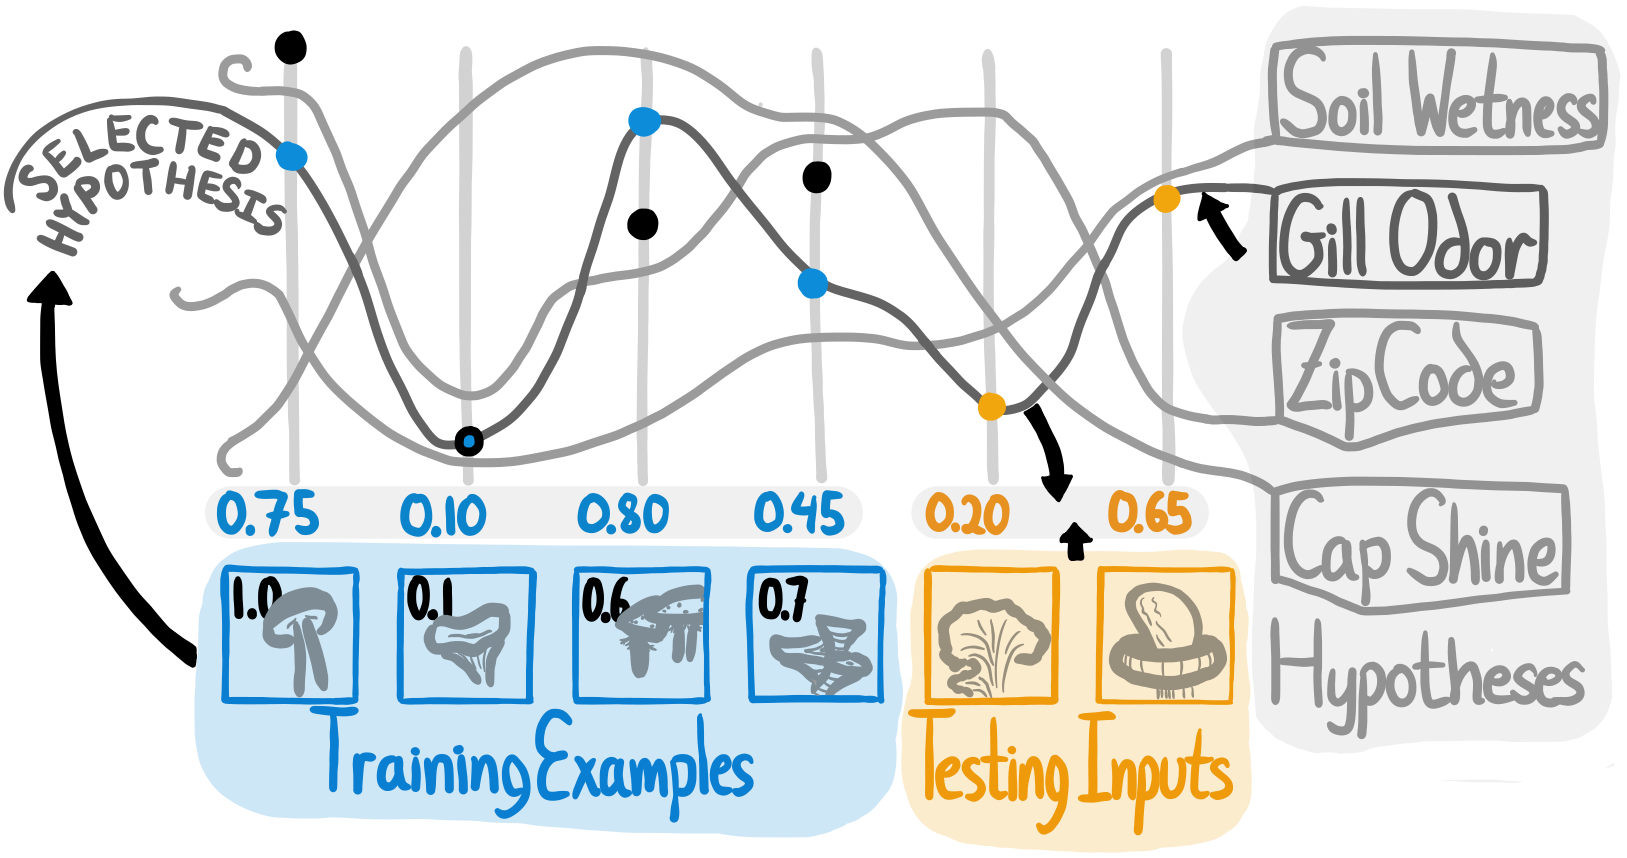
\includegraphics[width=\textwidth]{figures/ml-dataflow}
    \caption{%
      \textbf{Predicting mushrooms' poisons.}
      %
      Our learning program selects from a class of hypotheses ({\gre gray blob}) a plausible
      hypothesis that well fits (\textbf{\blu blue dots} are close to
      \textbf{black dots}) a given list of poison-labeled mushrooms ({\blu blue
      blob}).  Evaluating the selected hypothesis on new mushrooms, we predict
      the corresponding poison levels ({\rng orange numbers}).
      %
      \par The arrows show dataflow: how the hypothesis class and the
      mushroom+poisonlevel examples determine one hypothesis, which, together
      with new mushrooms, determines predicted poison levels.
      %
      Selecting a
      hypothesis is called \textbf{learning}; predicting unseen poison levels,
      \textbf{inference}.  The examples we learn from are
      \textbf{training data}; the new mushrooms and their true poison levels
      are \textbf{testing data}.
    }
    \vspace{-1.0cm}
  \end{figure}

  For example, say we want to predict poison levels (answers) of mushrooms
  (prompts).  %Comparing our `\textbf{training data}' to our
  Among our hypotheses,\bovinenote{%
      We choose four hypotheses: respectively, that
      a mushroom's poison level is
      close to:
      \par\emph{--- its ambient soil's percent water by weight};
      \par\emph{--- its gills' odor level, in kilo-Scoville units};
      \par\emph{--- its zipcode (divided by 100000)};
      \par\emph{--- the fraction of visible light its cap reflects}.
  }
  the GillOdor hypothesis fits the examples well: it guesses poison
  levels
  %(\textbf{\blu blue dots})
  close to the truth.
  %(\textbf{black dots}).
  So the program selects GillOdor.
 %(jargon: \textbf{learns})
  %The selection process is called \textbf{learning}.

  `\emph{Wait!}', you say,
  `\emph{doesn't Zipcode fit the example data more closely than GillOdor?'}.
  Yes.  But a poison-zipcode proportionality is implausible: we'd need
  more evidence before believing Zipcode.  We can easily make many oddball
  hypotheses; by chance some may fit our data well, but they probably
  won't predict well!
  %
  Thus
  ``intrinsic plausibility'' and ``goodness-of-fit-to-data''
  \emph{both}\bovinenote{%
    We choose those two notions (and our $\hH$) based on \textbf{domain
    knowledge}.  This design process is an art; we'll study some rules of
    thumb.
  } play a role in learning.

  %We must specify both notions based on our domain knowledge
  %--- this is an art but we'll learn its rules of thumb.
  %
  %We've now met ML's key elements.
  %Those are ML's elements.
  In practice we'll think of each hypothesis as mapping mushrooms to
  \emph{distributions} over poison levels; then its
  ``goodness-of-fit-to-data'' is simply the chance it allots to the
  data.\bovinenote{That's why we'll need \textbf{probability}.}
  %the details are more complex.
  We'll also use huge $\hH$s: we'll \emph{combine} mushroom features
  (wetness, odor, and shine) to make more hypotheses such as
  %Maybe
  $
    (1.0 \cdot \text{GillOdor} - 0.2\cdot \text{CapShine})
  $.\bovinenote{That's why we'll need \textbf{linear algebra}.}
  %predicts poison well!
  %
  Since we can't compute ``goodness-of-fit'' for so many hypotheses,
  we'll guess a hypothesis
  %start at a tentative hypothesis and
  then repeatedly
  nudge it up the ``goodness-of-fit'' \emph{slope}.\bovinenote{That's why we'll need \textbf{derivatives}.}
  %
  %

  %We must specify both notions based on our domain knowledge
  %--- this is an art but we'll learn its rules of thumb.
  %%
  %We'll often do this in terms of \emph{probabilities}:\bovinenote{%
  %  Still, probability isn't the only criterion: if overestimating poison
  %  levels is safer than underestimating them, then we'd want to hedge toward
  %  overestimating.
  %  This will become especially unavoidable when in Unit 5 we learn
  %  from reinforcement.
  %}
  %we supply a distribution over all hypotheses (a \textbf{prior}) and, we think
  %of each hypothesis as mapping mushrooms to \emph{distributions} over poison
  %levels.

  %\bovinenote{%
  %    \textbf{Bayesian Information Criterion}
  %}

\sampassage{supervised learning}
  We'll soon allow uncertainty by letting patterns map prompts to
  \emph{distributions} over answers.
  %\bovinenote{%
  %  Then learning programs have this type:
  %  $$
  %    \lL : (\xX\times \yY)^N \to (\xX\to \text{DistributionsOn}(\yY))
  %  $$
  %}
  %
  Even if there is only one prompt --- say, ``\emph{produce a
  beautiful melody}'' --- we may seek to learn the complicated
  distribution over answers, e.g.\ to generate a diversity of apt
  answers.  Such \textbf{unsupervised learning} concerns output
  structure.
  %
  By contrast, \textbf{supervised learning} (our main subject), concerns
  the input-output relation; it's interesting when there are many possible prompts.
  %there are many possible prompts.
  %
  Both involve learning from examples; the distinction is no more firm
  than that between sandwiches and hotdogs, but the words are good to
  know.

  %To save ink, say that $\xX$ is the set of possible prompts; $\yY$, of
  %possible answers.
  %%
  %With the example above, $\xX$ contains all
  %conceivable mushrooms and $\yY$ contains all conceivable poison
  %levels (perhaps all the non-negative real numbers).
  %%
  %If we like, we can now summarize the data flow in symbols.  A pattern is a
  %function of type $\xX\to\yY$.  And we can model the examples from which our
  %program learns as a list of type $(\xX\times \yY)^N$.  Then a program that
  %learns from examples has type:
  %$$
  %  \lL : (\xX\times \yY)^N \to (\xX\to \yY)
  %$$

%\sampassage{learning as...}
%  TODO
%    %
%\attnsam{
%    machine learning is like science.
%    %
%    machine learning is like automatic programming.
%    %
%    machine learning is like curve-fitting.
%    %%
%    three classic threads of AI
%    }

    \samsection{our first learning algorithm}
      \hypertarget{A2}{}
          \samsection{a tiny example: handwritten digit classification}
      \samquote{
        The learning process is something you can incite, literally incite, like a riot.
      }{audre lorde}

%~~~~~~~~~~~~~~~~~~~~~~~~~~~~~~~~~~~~~~~~~~~~~~~~~~~~~~~~~~~~~~~~~~~~~~~~~~~~~~
%~~~~~~~~~~~~~  1.3. meeting the data  ~~~~~~~~~~~~~~~~~~~~~~~~~~~~~~~~~~~~~~~~

      \sampassage{meeting the data}
        $\xX = \{\text{grayscale~}28\!\times\!28\text{-pixel images}\}$;
        $\yY=\{{\cya{1}},{\red{9}}\}$.  Each datum $(x,y)$ arises as follows:
        we randomly choose a digit $y\in \yY$, ask a human to write that digit
        in pen, and then photograph their writing to produce $x\in\xX$.
        %
        \vspace{-0.25cm}
        \begin{figure}
            \centering
          \begin{tabular}{c}
\includegraphics[width=0.75cm]{example-mnist/mnist-trn-00}\\$\red{9}$\\
\includegraphics[width=0.75cm]{example-mnist/mnist-trn-10}\\$\cya{1}$\end{tabular}%
          \begin{tabular}{c}
\includegraphics[width=0.75cm]{example-mnist/mnist-trn-01}\\$\cya{1}$\\
\includegraphics[width=0.75cm]{example-mnist/mnist-trn-11}\\$\red{9}$\end{tabular}%
          \begin{tabular}{c}
\includegraphics[width=0.75cm]{example-mnist/mnist-trn-02}\\$\red{9}$\\
\includegraphics[width=0.75cm]{example-mnist/mnist-trn-12}\\$\cya{1}$\end{tabular}%
          \begin{tabular}{c}
\includegraphics[width=0.75cm]{example-mnist/mnist-trn-03}\\$\red{9}$\\
\includegraphics[width=0.75cm]{example-mnist/mnist-trn-13}\\$\cya{1}$\end{tabular}%
          \begin{tabular}{c}
\includegraphics[width=0.75cm]{example-mnist/mnist-trn-04}\\$\cya{1}$\\
\includegraphics[width=0.75cm]{example-mnist/mnist-trn-14}\\$\red{9}$\end{tabular}%
          \begin{tabular}{c}
\includegraphics[width=0.75cm]{example-mnist/mnist-trn-05}\\$\red{9}$\\
\includegraphics[width=0.75cm]{example-mnist/mnist-trn-15}\\$\red{9}$\end{tabular}%
          \begin{tabular}{c}
\includegraphics[width=0.75cm]{example-mnist/mnist-trn-06}\\$\red{9}$\\
\includegraphics[width=0.75cm]{example-mnist/mnist-trn-16}\\$\red{9}$\end{tabular}%
          \begin{tabular}{c}
\includegraphics[width=0.75cm]{example-mnist/mnist-trn-07}\\$\red{9}$\\
\includegraphics[width=0.75cm]{example-mnist/mnist-trn-17}\\$\cya{1}$\end{tabular}%
          \begin{tabular}{c}
\includegraphics[width=0.75cm]{example-mnist/mnist-trn-08}\\$\cya{1}$\\
\includegraphics[width=0.75cm]{example-mnist/mnist-trn-18}\\$\red{9}$\end{tabular}%
          \begin{tabular}{c}
\includegraphics[width=0.75cm]{example-mnist/mnist-trn-09}\\$\red{9}$\\
\includegraphics[width=0.75cm]{example-mnist/mnist-trn-19}\\$\cya{1}$\end{tabular}%
          \caption{
            Twenty example pairs.  Each photo $x$ is a $28\times 28$ grid of
            numbers representing pixel intensities.  The light gray background
            has intensity $0.0$; the blackest pixels, intensity $1.0$.  Below
            each photo $x$ we display the corresponding label $y$:
            either $y= {\cya{1}}$ or
            $y={\red{9}}$.
            %
            We'll adhere to this color code throughout this tiny example.
          }
        \end{figure}

        \begin{marginfigure}
          \vspace{-3.5cm}
          
\includegraphics[width=0.47\textwidth]{example-mnist/mnist-trn-00}%\\$\red{9}$
            \hspace{0.03\textwidth}
          
\includegraphics[width=0.47\textwidth]{example-mnist/mnist-trn-01}%\\$\cya{1}$
        \end{marginfigure}
        When we zoom in, we can see each photo's $28\times 28$ grid of pixels.
        On the computer, this data is stored as a $28\times 28$ grid of
        numbers: $0.0$ for bright through $1.0$ for dark.  We'll name these
        $28\times28$ grid locations by their row number (counting starting from
        the top) followed by their column number (counting starting from the
        left).  So location $(0,0)$ is the upper left corner pixel; location
        $(27,0)$ is the lower left corner pixel.
        \par\noindent
        \attn{Exercise:} {Where is location $(0,27)$?  %$(14,8)$?
        In which direction is $(14,14)$ off-center?}


        As part of getting to know the data, it's worth taking a moment to
        think about how we would go about hand-coding a digit classifier.  The
        challenge is to complete the pseudocode
        %
        ``\texttt{if (?)\ then predict y=9 else predict y=1}''.
        %
        Well, ${\red{9}}$s tend to have more ink than than ${\cya{1}}$s ---
        should \texttt{(?)}\ threshold by the photo's darkness?
        %
        Or: ${\cya{1}}$s and ${\red{9}}$s tend to have different heights ---
        should \texttt{(?)}\ threshold by the photo's dark part's height?

        \begin{marginfigure}
          \centering
          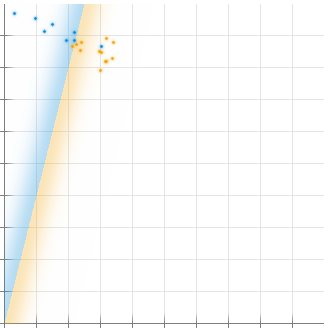
\includegraphics[width=0.99\textwidth]{example-mnist/train-plain}
            \vspace{-0.25cm}
          \caption{
            Our size-$N=25$ set of training examples, viewed in the
            darkness-height plane.  The vertical \emph{darkness} axis ranges
            $[0.0,0.25]$; the horizontal \emph{height} axis ranges $[0.0,0.5]$.
            The origin is at the lower left.  Each {\cya{cyan}} dot represents a
            $y={\cya{1}}$ example; each {\red{red}} dot, a $y={\red{9}}$ one.
            %
            The big ${\red{9}}$ above has darkness and height $(0.118, 0.375)$;\
            the big ${\cya{1}}$, $(0.092, 0.404)$.  See where they are in this
            plot?
          }
        \end{marginfigure}

        To make this precise, let's define a photo's \emph{darkness} as its
        average pixel darkness; its \emph{height} as the standard deviation of
        the row index of its dark pixels.  For convenience let's normalize
        both height and darkness to have max possible value $1.0$.  Such
        functions from inputs in $\xX$ to numbers are called
        \textbf{features}.

        \begin{lstlisting}[language=Python, basicstyle=\footnotesize\ttfamily]
          SIDE = 28
          def darkness(x):
            return np.mean(np.mean(x, axis=0), axis=0)
          def height(x):
            return np.std([row for col in range(SIDE)
                               for row in range(SIDE)
                               if 0.5 < x[row][col]  ])/(SIDE/2.0)
        \end{lstlisting}
        \par\noindent
        \attn{Exercise:} {Make a width feature.  Plot the training data
        in the height-width plane.}

        So we can threshold by darkness or by height.  But this isn't very
        satisfying, since sometimes there are especially dark ${\cya{1}}$s or
        tall ${\red{9}}$s.
        %
        We thus arrive at the idea of using \emph{both} features: ${\red{9}}$s
        are darker than ${\cya{1}}$s \emph{even relative to their
        height}.  So we might write something like
        \texttt{a*darkness(x)+b*height(x)>0} for
        %\bcirc\marginnote{%
        %  \blarr That factor of $2$ comes from our observation that darkness
        %  tends to be bigger than height.  We'll soon see that this eyeballed
        %  slope doesn't work well.  It's better to tune by machine.
        %}
        our condition.
        \par\noindent
        \attn{Exercise:} {Guess a good pair $(a,b)$ based on the training data.}
        \begin{lstlisting}[language=Python, basicstyle=\footnotesize\ttfamily]
          def hand_coded_predict(x):
            return 9 if (4.0)*darkness(x)+(-1.0)*height(x)>0 else 1
        \end{lstlisting}
        \par\noindent
        \attn{Exercise:} {Implement a crude ``hole-detector'' feature.  False
        positives are okay.}
        \par\noindent
        \attn{Exercise:} {What further features might help us to separate digits
        ${\cya{1}}$ from ${\red{9}}$?}

%~~~~~~~~~~~~~~~~~~~~~~~~~~~~~~~~~~~~~~~~~~~~~~~~~~~~~~~~~~~~~~~~~~~~~~~~~~~~~~
%~~~~~~~~~~~~~  1.4. candidate patterns  ~~~~~~~~~~~~~~~~~~~~~~~~~~~~~~~~~~~~~~

      \sampassage{candidate patterns}
        We can generalize the hand-coded hypothesis from the previous passage
        to other coefficients besides $1\cdot \text{height}(x) -
        2\cdot\text{darkness}(x)$.  We let our set $\hH$ of candidate patterns
        contain all ``linear hypotheses'' $f_{a,b}$ defined by:
        $$
          f_{a,b}(x) = {\red{9}} \text{~~if~~} a\cdot\text{darkness}(x) + b\cdot\text{height}(x) > 0 \text{~~else~~} {\cya{1}}
        $$
        Each $f_{a,b}$ makes predictions of $y$s given $x$s.  As we change $a$
        and $b$, we get different predictors, some more accurate than others.

        \begin{lstlisting}[language=Python, basicstyle=\footnotesize\ttfamily]
          def predict(x,a,b):
            return 9 if a*darkness(x) + b*height(x) > 0 else 1
        \end{lstlisting}

        \noindent
        \attn{Exercise:} {See Fig.\ \ref{fig:train-test-digits} and match up $\offourline{0}$'s $3$ lines with
        $\offourline{1}$'s $3$ boxed points.}

%~~~~~~~~~~~~~~~~~~~~~~~~~~~~~~~~~~~~~~~~~~~~~~~~~~~~~~~~~~~~~~~~~~~~~~~~~~~~~~
%~~~~~~~~~~~~~  1.5. optimization  ~~~~~~~~~~~~~~~~~~~~~~~~~~~~~~~~~~~~~~~~~~~~

      \sampassage{optimization}
        Let's write a program $\lL$ that given a list of \emph{training
        examples} produces a hypothesis in $h \in \hH$ that helps us predict
        the labels $y$ of yet-unseen photos $x$ (\emph{testing examples}).
        Insofar as training data is representative of testing data, it's
        sensible to return a $h\in \hH$ that correctly classifies maximally
        many training examples.
        %
        To do this, let's make $\lL$ loop over all integer pairs $(a,b)$ in
        $[-99,+99]$:  %to minimize the number of misclassified training examples.
        \begin{lstlisting}[language=Python, basicstyle=\footnotesize\ttfamily]
          def accuracy_on(examples,a,b):
            return sum(1.0 for x,y in examples if predict(x,a,b)==y)/len(examples)

          def best_hypothesis():
            return max((accuracy_on(training_data, a, b), (a,b))
                       for a in range(-99,100)
                       for b in range(-99,100))
        \end{lstlisting}

        \begin{figure}[h]
            \centering
            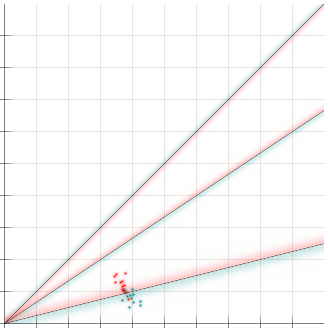
\includegraphics[width=0.23\textwidth]{example-mnist/new-train.png}%
            \hspace{0.01\textwidth}%
            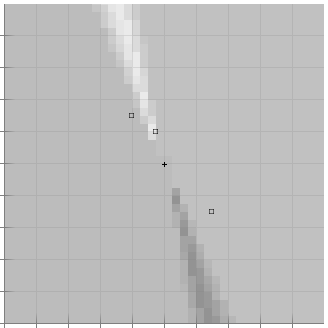
\includegraphics[width=0.23\textwidth]{example-mnist/new-train-scat.png}%
            \hspace{0.02\textwidth}%
            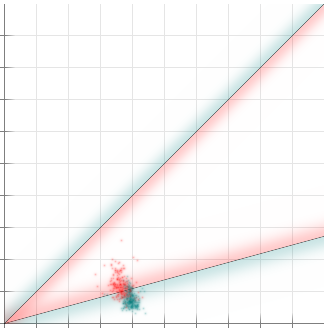
\includegraphics[width=0.23\textwidth]{example-mnist/new-test.png}%
            \hspace{0.01\textwidth}%
            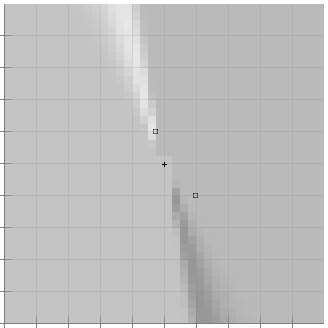
\includegraphics[width=0.23\textwidth]{example-mnist/new-test-scat.png}
            %
            \caption{
              \textbf{Training
              ($\protect\offourline{01}$) and testing
              ($\protect\offourline{23}$).}
              %
              $3$ hypotheses classify training data in the darkness-height
              plane ($\protect\offourline{0}$); glowing colors distinguish a
              hypothesis' $\cya{1}$ and $\red{9}$ sides.
              %
              Each point in the $(a,b)$ plane ($\protect\offourline{1}$)
              represents a hypothesis; darker regions misclassify a greater
              fraction of training data.
              %
              Panes $\protect\offourline{23}$ show the same for
              \emph{testing} data.
              %
              $\protect\offourline{02}$'s axes range $[0, 1.0]$.
              $\protect\offourline{13}$'s axes range $[-99,+99]$.
            }
            \label{fig:train-test-digits}
        \end{figure}


        When we feed $N=25$ training examples to $\lL$, it produces
        $(a,b)=(80,-20)$ as a minimizer of \textbf{training error}, i.e.,
        of the fraction of training examples misclassified.  It misclassifies
        only $12\%$ of training examples. Yet the same
        hypothesis misclassified a greater fraction --- $18\%$ --- of fresh,
        yet-unseen testing examples.
        %
        That latter number --- called the \textbf{testing error} --- represents
        our program's accuracy ``in the wild'';
        it's the number we most care about.  The difference between training
        and testing error is the difference between our score on a practice
        exam or homework, where we're allowed to review mistakes we made and
        do a second try, versus our score on an exam, where we don't know the
        questions beforehand and aren't allowed to change our answers once we
        get our grades back.

        \noindent
        \attn{Exercise:} {visualize $f_{a,b}$'s error on $N=1$ example as a
        function of $(a,b)$.}



    \samsection{how well did we do?  (3 kinds of error : opt, approx, gen)}
      \hypertarget{A2}{}
      \objectives{%
      \item compute and conceptually distinguish training and testing misclassification errors
      \item explain how the problem of achieving low testing error
            decomposes into the three problems of achieving low
            \emph{generalization},
            \emph{optimization}, and
            \emph{approximation}
            errors.
}

\sampassage{error analysis}
  Intuitively, our testing error of $17\%$ comes from three sources:
  \textbf{(a)} the failure of our training set to be representative of our testing set;
  \textbf{(b)} the failure of our program to exactly minimize training error over $\hH$; and
  \textbf{(c)} the failure of our hypothesis set $\hH$ to contain ``the true'' pattern.

  These are respectively errors of
  \textbf{generalization},
  \textbf{optimization},
  \textbf{approximation}.

  We can see generalization error when we plot testing data in the
  brightness-width plane.  The hypotheses $h=(20, 83)$ that we selected based
  on the training in the brightness-width plane misclassifies many testing
  points.  we see many misclassified points.  Whereas $h$ misclassifies only
  $10\%$ of the training data, it misclassifies $17\%$ of the testing data.
  This illustrates generalization error.

  In our plot of the $(a,b)$ plane,
  the {\blu blue square} is the hypothesis $h$ (in $\hH$) that best fits
  the training data.  The {\rng orange square} is the hypothesis (in
  $\hH$) that best fits the testing data.  But even the latter seems
  suboptimal, since $\hH$ only includes lines through the origin while it
  seems we want a line --- or curve --- that hits higher up on the
  brightness axis.  This illustrates approximation error.\bovinenote{%
    To define \emph{approximation error}, we need to specify whether the `truth'
    we want to approximate is the training or the testing
    data.  Either way we get a useful concept.  In this paragraph we're talking
    about approximating \emph{testing} data; but in our notes overall we'll
    focus on the concept of error in approximating \emph{training} data.
  }

  Optimization error is best seen by plotting training rather than testing
  data.  It measures the failure of our selected hypothesis $h$ to minimize
  training error --- i.e., the failure of the {\blu blue square} to lie in a
  least shaded point in the $(a,b)$ plane, when we shade according to training
  error.

  \begin{figure}[h]
  %\begin{marginfigure}%[h]
      \centering
      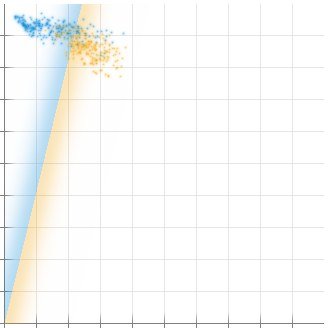
\includegraphics[width=0.49\textwidth]{example-mnist/test-features.png}%
      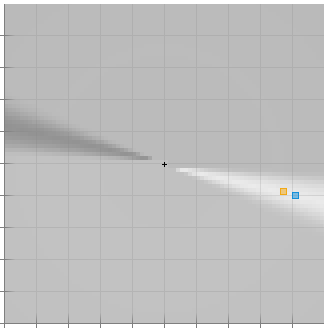
\includegraphics[width=0.49\textwidth]{example-mnist/test-weights.png}%
      %
      \caption{
          \textbf{Testing error visualized two ways.}.
        --- %  \par\noindent
        \textbf{Left: in feature space.}
        The hypotheses $h=(20, 83)$ that we selected based on the training set
        classifies testing data in the brightness-width plane; glowing colors
        distinguish a hypothesis' $\blu{1}$ and $\rng{3}$ sides.
        Axes range $[0, 1.0]$.
        %
        %
        --- %  \par\noindent
        \textbf{Right: in weight space.}
        %
        Each point in the $(a,b)$ plane
        represents a hypothesis; darker regions misclassify a greater
        fraction of testing data.  Axes range $[-99,+99]$.
        %
      }
      \label{fig:test-features-weights}
  \end{figure}
  %\end{marginfigure}

  Here, we got optimization error $\approx 0\%$ (albeit by
  \emph{unscalable brute-force}).  Because optimization error is zero in
  our case, the approximation error and training error are the same:
  $\approx10\%$.  The approximation error is so high because our straight
  lines are \emph{too simple}: brightness and width lose useful
  information and the ``true'' boundary between digits --- even training ---
  may be curved.
  %
  Finally, our testing error $\approx 17\%$ exceeds our training error.
  We thus suffer a generalization error of $\approx 7\%$: we \emph{didn't
  perfectly extrapolate} from training to testing situations.
  %
  In 6.86x we'll address all three italicized issues.

  \exercise{why is generalization error usually positive?}



\sampassage{formalism}\marginnote{\veryoptional}
  Here's how we can describe learning and our error decomposition in
  symbols.
  %
  Draw training examples $\sS : (\xX\times \yY)^N$
  from nature's distribution $\dD$ on $\xX\times \yY$.  A hypothesis
  $f:\xX\to \yY$ has \textbf{training error}
  $
     \Ein(f) = \Pp_{(x,y)\sim \blu{\sS}}[f(x)\neq y]
  $, an average over examples; and \textbf{testing error}
  $
     \Eout(f) = \Pp_{(x,y)\sim \rng{\dD}}[f(x)\neq y]
  $, an average over nature.  A \emph{learning program} is a function
  $
      \lL : (\xX\times \yY)^N \to (\xX\to \yY)
  $; we want to design $\lL$ so that it maps typical $\sS$s to $f$s with
  low $\Eout(f)$.
  %\marginnote{%
  %  %  TODO: mention extereme class-imbalance and bayesian *decision* theory
  %}

  So
  we often define
  $\lL$ to roughly
  minimize $\Ein$ over a
  set $\hH \subseteq (\xX\to \yY)$ of candidate patterns.  Then $\Eout$
  decomposes
  into the failures
  of
  $\Ein$ to estimate $\Eout$ (generalization),
  of
  $\lL$ to minimize $\Ein$ (optimization), and
  of
  $\hH$ to contain
  nature's
  truth (approximation):
  \newcommand{\minf}[1]{{\inf}_{\hH}}
  \begin{align*}
      \Eout(\lL(\sS))
      =~&\Eout(\lL(\sS))      &-\,\,\,&      \Ein(\lL(\sS)) &~\}~~& \text{\textbf{generalization} error} \\
      +~&\Ein(\lL(\sS))       &-\,\,\,& \minf{\hH}(\Ein(f)) &~\}~~& \text{\textbf{optimization} error} \\
      +~&\minf{\hH}(\Ein(f))  &       &                     &~\}~~& \text{\textbf{approximation} error}
  \end{align*}
  These terms are in tension.  For example, as $\hH$ grows, the
  approx.\ error may decrease while the gen.\ error may
  increase --- this is the ``\textbf{bias-variance} tradeoff''.

    \samsection{how can we do better?  (survey of rest of notes)}
      \hypertarget{A2}{}
      
%~~~~~~~~~~~~~~~~~~~~~~~~~~~~~~~~~~~~~~~~~~~~~~~~~~~~~~~~~~~~~~~~~~~~~~~~~~~~~~
%~~~~~~~~~~~~~  1.9. workflow  ~~~~~~~~~~~~~~~~~~~~~~~~~~~~~~~~~~~~~~~~~~~~~~~~

%      \sampassage{workflow}
%      %\sampassage{workflow: framing}
%        We first \emph{frame}: what data will help us solve what problem?  To
%        do this, we \emph{factor} our complex prediction problem into simple
%        classification or regression problems; randomly \emph{split} the
%        resulting example pairs into training, dev(elopment), and testing sets;
%        and \emph{visualize} the training data to weigh our intuitions.
%
%      %\sampassage{workflow: modeling}
%        Next, we \emph{model}: we present the data to the computer so that
%        true patterns are more easily found.
%        %
%        Here we inject our \emph{domain knowledge} --- our human experience and
%        intuition about which factors are likely to help with prediction.
%        %
%        Modeling includes \emph{featurizing} our inputs and choosing
%        appropriate \emph{priors} and \emph{symmetries}.
%
%      %\sampassage{workflow: training}
%        During \emph{training}, the computer searches among candidate patterns
%        for one that explains the examples relatively well.
%        We used brute force above; we'll soon learn faster algorithms
%        such as \emph{gradient descent} on the training set for parameter
%        selection and \emph{random grid search} on the dev set for
%        hyperparameter selection.
%
%      %\sampassage{workflow: harvesting}
%        Finally, we may \emph{harvest}: we derive insights from the pattern
%        itself\bovinenote{%
%            which factors ended up being most important?
%        }
%        and we predict outputs for to fresh inputs.
%        %
%        Qualifying both applications is the pattern's quality.  To assess this,
%        we measure its accuracy on our held-out testing data.




  \sampart{B. auto-predict by fitting lines to examples (unit 1)}
    \phantomsection\label{part:B}
    \samsection{linear approximation}
      \hypertarget{B0}{}
      %==============================================================================
%====  2.  LINEAR MODELS BASICS  =============================================
%==============================================================================

  %\sampart{B. linear models}\label{chap:linear}
  \sampart{B. linear classification}\label{chap:linear}

    \samsection{0. linear approximations}
      \samquote{
        He had bought a large map representing the sea, \\
        Without the least vestige of land: \\
        And the crew were much pleased when they found it to be \\
        A map they could all understand.
      }{charles dodgson}

%~~~~~~~~~~~~~~~~~~~~~~~~~~~~~~~~~~~~~~~~~~~~~~~~~~~~~~~~~~~~~~~~~~~~~~~~~~~~~~
%~~~~~~~~~~~~~  2.0. featurization  ~~~~~~~~~~~~~~~~~~~~~~~~~~~~~~~~~~~~~~~~~~~

      \sampassage{featurization}  % as an art of
        As in the prologue, we represent our input $x$ as a fixed-length list
        of numbers so that we can treat $x$ with math. 
        There, we
        represented each photograph by $2$ numbers: height and darkness.  We
        could instead have represented each photograph by $784$ numbers, one
        for the brightness at each of the $28\cdot 28=784$ many pixels.  Or by
        $10$ numbers, each measuring the overlap of $x$'s ink with that of
        ``representative'' photos of the digits $0$ through $9$.

        When we choose how to represent $x$ by a list of numbers, %
        we're
        choosing a \textbf{featurization}.  We call each number a ``feature''.
        For example, height and darkness are two features.

        %``height'' and ``darkness'' are \emph{features}: maps $\xX\to \Rr$ used
        %to pre-process $x$s.

        \attnsam{TODO: mention one-hot, etc}
        \attnsam{TODO: mention LOWRANK (sketching; also, for multiregression)}
        %
        There are lots of interesting featurizations, each making different
        patterns easier to learn.\marginnote{%
            \attnsam{data-based featurizations via kernels}
            \attnsam{will soon learn featurizations}
            \attnsam{hand featurization in kaggle and medicine}
        }
        We judge a featurization not in a vacuum but with respect to
        the kinds of patterns we use it to learn. %
        \attnsam{TODO: graphic of separability; and how projection can reduce it}
        Learning usually happens
        more accurately, robustly, and interpretably when our featurization is
        abstract (no irrelevant details) but complete (all relevant details),
        compressed (hard to predict one feature from the others) but accessible
        (easy to compute interesting properties from features).

        Here are three featurizations ideas that might inspire you in
        your own projects.

        \emph{Hardcoded coordinate transforms}.
        %
        \textbf{The bias trick}.\bcirc\marginnote{
            \blarr a.k.a.\ \textbf{projectivization}
        }
        We send
        $x \mapsto (1, x)$, thus increasing dimension by one.
        %\attnsam{TODO: projectivization (say this foreshadows kernel discussion?)}
        %
        \par
        Generalizing the above, we can
        use \textbf{polynomial features}:
        $$
            x \mapsto (x^{\otimes 0}, x^{\otimes 1}, \cdots, x^{\otimes d})
        $$
        By $x^{\otimes d}$, we mean a multiaxis array $a$ with $d$ axes and
        defined (in an example where $d=3$) by
        $$
            a_{42,686,0} = x_{42} x_{686} x_0 \in \Rr
        $$
        Note that this featurization is redundant since permuting $a$'s axes
        doesn't change $a$.
        %
        \par
        \textbf{coordinate transforms} --- e.g.\ arctan.

        \emph{Encoding the discrete}.
        \textbf{one-hot}
        %
        \par
        \textbf{Binning}

        \emph{Data-dependent transforms}.
        %
        \textbf{Quantilization}
        %
        \par
        \textbf{Landmarks}

        %In the exercise at the end of the passage on ``meeting the data'', we
        %dreamed up other ``features'' (besides \emph{height} and
        %\emph{darkness}) that might help to distinguish ${\red{9}}$s
        %from ${\cya{1}}$s.
        %%
        %Maybe we thought of \emph{width}.  Or of whether the ink surrounds a
        %\emph{hole}, as in a ${\red{9}}$.  Or of a photo's \emph{topheaviness}:
        %is its top half darker than its bottom half?  We might have chosen a
        %`canonical' photo of each of the digits in order to consider how a
        %given photo's ink \emph{overlaps} with those canonical photos'.
        %%
        %These are just some of very many good ideas.

        %Let's crudely define a photo as having a \emph{hole} at location
        %$(r,c)$ when, for each quadrant around $(r, c)$, location
        %$(r,c)$ is strictly brighter than a location in that quadrant.  A
        %photo's \emph{holiness} is the fraction of its pixels that are holes.

        %And let's define the \emph{overlap} between two photos as the fraction
        %of their pixels that are both above or both below $0.5$ in darkness.

        %\begin{lstlisting}[language=Python, basicstyle=\footnotesize\ttfamily]
        %  SIDE = 28
        %  def darkness(x):
        %    return np.mean(np.mean(x))
        %  def height(x):
        %    return np.std([row for col in range(SIDE)
        %                       for row in range(SIDE)
        %                       if 0.5 < x[row][col]  ])/(SIDE/2.0)
        %  def width(x):
        %    return np.std([row for col in range(SIDE)
        %                       for row in range(SIDE)
        %                       if 0.5 < x[row][col]  ])/(SIDE/2.0)
        %  def holiness(x):
        %    return np.mean([1 if (np.max(x[:row,:col]) > x[row,col] and
        %                          np.max(x[:row,col:]) > x[row,col] and
        %                          np.max(x[row:,:col]) > x[row,col] and
        %                          np.max(x[row:,col:]) > x[row,col]    ) else 0
        %                      for col in range(1,SIDE-1)
        %                      for row in range(1,SIDE-1)                       ])
        %  def topheaviness(x):
        %    return (np.mean(x[:int(SIDE/2)])-np.mean(x[int(SIDE/2):]) + 1.0)/2
        %  #def overlap_one(x):
        %  #  return np.sum()
        %  #def overlap_nine(x):
        %\end{lstlisting}
        %We normalized all features so that they output values in $[0.0,1.0]$.

        %\par\noindent
        %\attn{Exercise:} {How might our ${\red{9}}$ vs ${\cya{1}}$ model fail
        %to generalize to photos of unevenly lit paper?  Photos of lined paper?
        %Of chalk on slate?  Of $7$-segment digital displays?
        %\par\noindent
        %\attn{Exercise:} {How might they fail for classifying $3$ vs $8$?}
%~~~~~~~~~~~~~~~~~~~~~~~~~~~~~~~~~~~~~~~~~~~~~~~~~~~~~~~~~~~~~~~~~~~~~~~~~~~~~~
%~~~~~~~~~~~~~  2.1. geometry of feature-space  ~~~~~~~~~~~~~~~~~~~~~~~~~~~~~~~

      \sampassage{geometry of feature-space} % pictures!
        Say we've decided on a \textbf{featurization} of our input
        data $x$.
        %$$
        %  f_{a,b}(x) = ~0 \text{~~if~~} a\cdot \text{width}(x) + b\cdot\text{darkness}(x) < 0 \text{~~else~~} 1
        %$$
        \begin{marginfigure}
          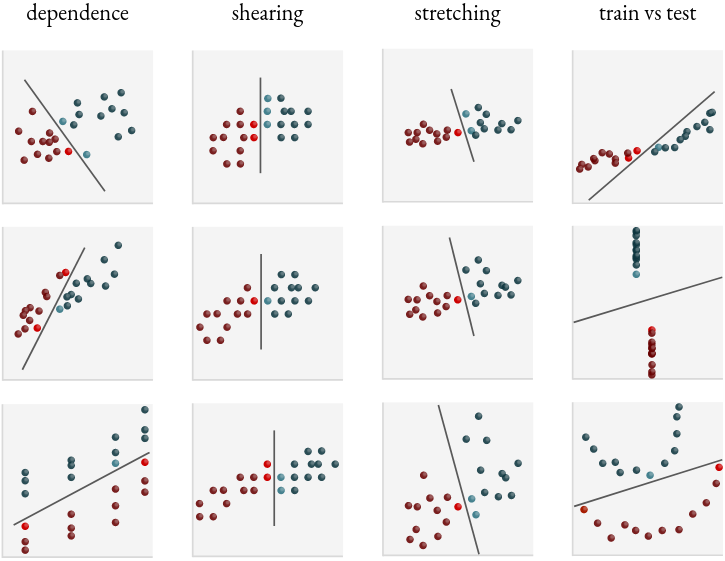
\includegraphics[width=\textwidth]{feature-space-phenomena}
        \end{marginfigure}

        % dependence
        Just because two features both correlate with a positive label ($y=+1$)
        doesn't mean both features will have positive weights.  In other words,
        it could be that the \emph{blah}-feature correlates with $y=+1$ in the
        training set and yet, according to the best hypothesis for that
        training set, the bigger a fresh input's blah feature is, the
        \emph{less} likely its label is to be $+1$, all else being equal.  That
        last phrase ``all else being equal'' is crucial, since it refers to our
        choice of coordinates.
        %
        \attnsam{Illustrate `averaging' of good features vs `correction' of one
        feature by another (how much a feature correlates with error)}
        %
        In fact, t This is the difference between \emph{independence} and
        \emph{conditional independence}.

        % shearing
        Shearing two features together --- e.g.\ measuring
        cooktime-plus-preptime together with cooktime rather than preptime
        together with cooktime --- can impact the decision boundary.
        %
        Intuitively, the more stretched out a feature axis is, the more the
        learned hypothesis will rely on that feature.

        % stretching
        Stretching a single feature --- for instance, measuring it in
        centimeters instead of meters --- can impact the decision boundary
        as well.  Intuitively, the more stretched out a feature axis is,
        the more the learned hypothesis will rely on that feature.

        % train vs test
        Note that

        %Caution: a feature $A(\sfx)$ that is statistically independent from
        %$\sfy$ may still be relevant for predicting $\sfy$.\marginnote{%
        %  Example.  Consider the uniform distribution on the four corners of a
        %  tetrahedron embedded within the corners of a cube \attnsam{TODO:
        %  graphic}.  The three spatial coordinates give three bit-valued random
        %  variables.  Any two of these variables are independent.  But the
        %  three together are dependent.
        %  \attnsam{TODO: also do a decision boundary (simpsons style) graph
        %  illustrating this phenomenon}
        %}
        %For example, if
        %$A, B$ are two features, it is possible that $A(\sfx), \sfy$ are
        %independent and that $B(\sfx), \sfy$ are independent and yet
        %$A(\sfx),B(\sfx), \sfy$ are \emph{dependent}!

        \attnsam{TODO: example featurization (e.g. MNIST again?)}

%~~~~~~~~~~~~~~~~~~~~~~~~~~~~~~~~~~~~~~~~~~~~~~~~~~~~~~~~~~~~~~~~~~~~~~~~~~~~~~
%~~~~~~~~~~~~~  2.2. richer outputs  ~~~~~~~~~~~~~~~~~~~~~~~~~~~~~~~~~~~~~~~~~~

      %\sampassage{richer outputs: larger $\yY$}
      \sampassage{more classes and beyond}
        We've learned how to construct a set $\hH$ of candidate patterns
        $$
          f_{\vec w}(\vec x) = \text{step}(\vec w\cdot \vec x)
        $$
        that map (a featurization of) a prompt $\vec x$ to a binary answer
        $y=0$ or $y=1$.

        What if we're interested in predicting a richer kind of $y$?  For
        example, maybe there are $k$ many possible values for $y$ instead of
        just $2$.  Or maybe there are infinitely many possible values --- say,
        if $y$ is a real number or a length-$k$ list of real numbers.  Or maybe
        we want the added nuance of predicting probabilities, so that $f$ might
        output ``19\% chance of label $y=0$ and 80\% chance of label $y=1$ and
        1\% chance of label $y=2$''
        instead of just ``$y=1$''.

        I'll write formulas and then explain.
        \begin{align*}
            \text{multi-class hard classification}\quad&
            f_{(\vec w_i : 0\leq i < k)}(\vec x) = \text{argmax}_i(\vec w_i\cdot \vec x : 0\leq i<k)
        \\
            \text{multi-output regression}\quad&
            f_{(\vec w_i  : 0\leq i < k)}(\vec x) = (\vec w_i \cdot \vec x : 0\leq i < k)
        \\
            \text{multi-class soft classification}\quad&
            f_{(\vec w_i  : 0\leq i < k)}(\vec x) = \text{normalize}(\exp(\vec w_i \cdot \vec x) : 0\leq i < k)
        \end{align*}

        A key ideas here is \emph{symmetry between classes}.  Previously, we
        interpreted positive decision function values as meaning one class and
        negative values as meaning the other.  This is asymmetrical --- why
        should one class count as positive?! --- and does not immediately
        generalize to multiple classes.
        %
        Instead, let's do two-class classification by producing \emph{two}
        values: the degree to which a point is of one class
            and the degree to which a point is of the other class.
        Then we'll classify according to which value is \emph{greater}.
        This is redundant because we could add $+42$ to both values and get the
        same answer for all inputs.  Redundancy is often the cost of symmetry.

        More generally, if we have three classes \emph{ostrich}, \emph{emu},
        and \emph{roc}, then we compute three linear functions representing
        \emph{ostrich-ness}, \emph{emu-osity}, and \emph{roc-iness}.  And we
        return whichever class has a greatest value.  This explains the
        \emph{multi-class hard classification}.

        For \emph{multi-output regression}, let's just skip the argmax.

        For \emph{multi-output soft classification}, we want to report
        probabilities instead of general real-valued scores.  Probabilities
        ought to be non-negative and ought to sum to one.  A nice way to turn
        general numbers to non-negative (in fact, positive) ones is to apply
        $\exp$.  A nice way to get positive numbers to sum to $1$ is to divide
        by their sum.  This leads us to \textbf{softmax}:
        $$
          \text{softmax}(\omega_k ~:~ 0\leq k<K) = \left(\frac{\exp(\omega_k)}{\sum_{k^\prime} \exp(\omega_{k^\prime})} ~:~ 0\leq k<K\right)
        $$

        %\attnsam{TODO: interpret}
        \attnsam{TODO: show pictures of 3 classes, 4 classes (e.g. digits 0,1,8,9)}
        %\attnsam{TODO: discuss measures of goodness!}
        \attnsam{TODO: talk about structured (trees/sequences/etc) output!}

%~~~~~~~~~~~~~~~~~~~~~~~~~~~~~~~~~~~~~~~~~~~~~~~~~~~~~~~~~~~~~~~~~~~~~~~~~~~~~~
%~~~~~~~~~~~~~  2.3. richer outputs  ~~~~~~~~~~~~~~~~~~~~~~~~~~~~~~~~~~~~~~~~~~

      \sampassage{visualizing high dimensional spaces}
        \attnsam{FILL IN}



        %-- what it means for "dogness vs catness" to vary linearly
        %-- log probabilities as the thing-to-approximate
        %-- humble models (svm, perceptron, etc)
        %-- richer outputs : regression and adt structure
    \samsection{iterative optimization}
      \hypertarget{B1}{}
          \newpage
    \samsection{1. iterative optimization}
      \samquote{
        Hey Jude, don't make it bad \\
        Take a sad song and make it better \\
        Remember to let her under your skin \\
        Then you'll begin to make it \\
        Better, better, better, better, better, better, ...
      }{paul mccartney, john lennon}

%~~~~~~~~~~~~~~~~~~~~~~~~~~~~~~~~~~~~~~~~~~~~~~~~~~~~~~~~~~~~~~~~~~~~~~~~~~~~~~
%~~~~~~~~~~~~~  2.4. stochastic gradient descent  ~~~~~~~~~~~~~~~~~~~~~~~~~~~~~

      \sampassage{(stochastic) gradient descent}
        We have a collection $\hH$ of candidate patterns together with a
        function $1-\Ein$ that tells us how good a candidate is.\marginnote{%
          $\leftarrow$ We view $1-\Ein$ as an estimate of our actual notion of
          ``good'': $1-\Eout$.
        }
        %
        In \S A we found a nearly best candidate by brute-force search over all
        of $\hH$; this doesn't scale to the general case, where $\hH$ is
        intractably large.
        %
        So: \emph{what's a faster algorithm to find a nearly best candidate?}

        A common idea is to start arbitrarily with some $h_0\in \hH$ and
        repeatedly improve to get $h_1, h_2, \cdots$.  Two questions are:
        \emph{how do we select $h_{t+1}$ in terms of $h_t$}?  And \emph{how do
        we know when to stop}?  We'll discuss termination conditions later
        --- for now, let's agree to stop at $h_{10000}$.

        As for selecting a next candidate, we'd like to use more detailed
        information on $h_t$'s inadequacies to inform our proposal $h_{t+1}$.
        Intuitively, if $h_t$ misclassifies a particular $(x_n, y_n) \in \sS$,
        then we'd like $h_{t+1}$ to be like $h_t$ but nudged a bit in the
        direction of accurately classifying $(x_n, y_n)$.

        Derivatives measure how changing a parameter a bit affects a result.
        So let's
        %
        \attnsam{FILL IN FOR PROBABILITIES (LOGISTIC) MODEL}

        This is the idea of \textbf{gradient descent}.
        \attnsam{MOTIVATE AND GIVE PSEUDOCODE FOR STOCHASTIC GD}

        Given a list of training examples, a probability model, and a
        hypothesis $\vec w$, we can compute $\vec w$'s asserted probability
        that the training $x$s correspond to the training $y$s.  It seems
        reasonable to choose $\vec w$ so that this probability is maximal.
        This method is called \textbf{maximum likelihood estimation (MLE)}.

%~~~~~~~~~~~~~~~~~~~~~~~~~~~~~~~~~~~~~~~~~~~~~~~~~~~~~~~~~~~~~~~~~~~~~~~~~~~~~~
%~~~~~~~~~~~~~  2.5. logistic models  ~~~~~~~~~~~~~~~~~~~~~~~~~~~~~~~~~~~~~~~~~

      \sampassage{logistic models} %``soft''

        The probability of a bunch of independent observations is the same as
        the product of probabilities of the observations.  Taking logarithms
        turns products into more manageable sums.  And --- this is a historical
        convention --- we further flip signs $\pm$ to turn maximization to
        minimization.
        %
        After this translation, MLE with the logistic model means finding $\vec
        w$ that minimizes
        $$
          \sum_i \log_2(1+\exp(-y_i\vec w\cdot \vec x_i))
          =
          \sum_i \text{softplus}(-y_i\vec w\cdot \vec x_i)
        $$
        Here, $\text{softplus}$ is our name for the function that sends
        $z$ to $\log_2(1+\exp(z))$.

        \attnsam{mention convexity and convergence?}
        \attnsam{show trajectory in weight space over time -- see how certainty
        degree of freedom is no longer redundant? (``markov'')}

%~~~~~~~~~~~~~~~~~~~~~~~~~~~~~~~~~~~~~~~~~~~~~~~~~~~~~~~~~~~~~~~~~~~~~~~~~~~~~~
%~~~~~~~~~~~~~  2.6. humble models  ~~~~~~~~~~~~~~~~~~~~~~~~~~~~~~~~~~~~~~~~~~~

      \newpage
      \sampassage{humble models}
        Let's modify logistic classification to allow for \emph{unknown
        unknowns}. We'll do this by allowing a classifier to allot probability
        mass not only among labels in $\yY$ but also to a special class $\star$
        that means ``no comment'' or ``alien input''.  A logistic classifier
        always sets $\Pp_{\sfy|\sfx}[\star|x] = 0$.
        %
        Other probability models may put nonzero mass on ``no comment'';
        different models give different learning programs.  Here are four
        models we might consider:
        \newcommand{\zp}{u^{\!+\!}}
        \newcommand{\zm}{u^{\!-\!}}
        \begin{table}
          \centering
          \small
          \vspace{-0.3cm}
          \begin{tabular}{RCCCC}
                                        & \textsc{logistic}     & \textsc{perceptron}       & \textsc{svm}              & \textsc{gauss-gen}        \\\hline %& \textsc{gauss}
            \Pp_{\sfy|\sfx}[-1| x]      & \zm/(\zm+\zp)         &\zm\cdot(\zm\wedge\zp)/2   &\zm\cdot(\zm/e\wedge\zp)/2 &\zm\cdot\text{bumps}       \\       %&\zm \cdot \epsilon e^{-d^2/4}
            \Pp_{\sfy|\sfx}[+1| x]      & \zp/(\zm+\zp)         &\zp\cdot(\zm\wedge\zp)/2   &\zp\cdot(\zm\wedge\zp/e)/2 &\zp\cdot\text{bumps}       \\       %&\zp \cdot \epsilon e^{-d^2/4}
            \Pp_{\sfy|\sfx}[\star| x]   & 1 - ~\text{above}=0   &1 - ~\text{above}          &1 - ~\text{above}          &1 - ~\text{above}          \\\hline %&1 - ~\text{above}
            %                                                                                                                                                %
            \text{loss name}            &\text{softplus}(\cdot) &\text{srelu}(\cdot)        &\text{hinge}(\cdot)        &\text{quad}(\cdot)         \\       %&\text{parab}(\cdot)
            \text{formula}              &\log_2(1+e^{(\cdot)})&\max(1,\cdot)+1            &\max(1,\cdot+1)            & ??                        \\       %&(\cdot+1)^2
            \text{update}               &1/(1+e^{+yd})        &\text{step}(-yd)           &\text{step}(1-yd)          & ??                        \\\hline %&2(1-yd)
            %                                                                                                                                                %
            \text{outliers}             &\text{robust-ish}      &\text{robust}              &\text{robust}              &\text{vulnerable}          \\       %&\text{vulnerable}
            \text{inliers}              &\text{sensitive}       &\text{blind}               &\text{sensitive}           &\text{blind-ish}           \\       %&\text{blind}
            \text{humility}             &\text{low}             &\text{low}                 &\text{high-ish}            &\text{high}                \\ 
            \text{acc bnd}              &\text{good}            &\text{bad}                 &\text{good}                &\text{good-ish}
            %\text{humility}             &\text{low}             &\text{medium}              &\text{high}                \\             % &\text{high}
            % TODO: split outliers/inliers by good or bad (erroneously classified or not?)  so 4 rows instead of 2?
          \end{tabular}
          \caption{%
            \textbf{Four popular models for binary classification.}
            %
            \textbf{Top rows:} Modeled chance given $x$ that $y=+1$ or $-1$ or
            $\star$.  We use $d = \vec w\cdot \vec x$, $u^{\!\pm\!}$ =
            $e^{\!\pm\! d/2}$, $a\wedge b = \min(a,b)$ to save ink.  And
            $\text{bumps}=(\phi(d-1)+\phi(d+1))/2$ with $\phi(\cdot)$ the
            standard normal density function.
            %
            \textbf{Middle rows:} neg-log-likelihood losses.
            %that arise when maximize likelihood using these models.
            An SGD step looks like
            $
              \vec w_{t+1} = \vec w_t + (\eta \cdot \text{update} \cdot y \vec x)
            $.
            %
            \textbf{Bottom rows:} All models respond to misclassifications.
            But are they robust
            to well-classified outliers?
            Sensitive to well-classified inliers?
            \par\noindent
            \attn{Exercise}: {
               Fill in the ??s in the rightmost column of the table above.
            }
          }
          \vspace{+0.3cm}
        \end{table}

        MLE with the perceptron model, svm model, or gauss-gen model minimizes
        the same thing, but with
        $\text{srelu}(z) = \text{max}(0,z)+1$,
        $\text{hinge}(z) = \text{max}(0,z+1)$, or
        $\text{quad}(z) = \cdots$
        instead of $\text{softplus}(z)$.\bcirc\marginnote{%
          \blarr Other models we might try will induce other substitutes for softplus.
          E.g.  $z\mapsto \text{hinge}(z)^2$ or $z\mapsto
          \text{avg}(z, \sqrt{z^2+4})$.
        }
        %https://www.desmos.com/calculator/3yak0ozell

        Two essential properties of $\text{softplus}$ are that:
        (a) it is convex and
        (b) it upper bounds the step function.
        Note that $\text{srelu}$, $\text{hinge}$, and $\text{quad}$ also enjoy
        these properties.  Property (a) ensures that the optimization problem
        is relatively easy --- under mild conditions, gradient descent is
        guaranteed to find a global minimum.  By property (b), the total loss
        on a training set upper bounds the rate of erroneous classification on
        that training set.  So loss is a \emph{surrogate} for (in)accuracy: if
        the minimized loss is nearly zero, then the training accuracy is nearly
        $100\%$.\marginnote{%
          The perceptron satisfies (b) in a trivial way that yields a trivial
          bound of $100\%$ on the error rate.
        }

        \attnsam{training behavior!!}
        \attnsam{response to outliers}
        \attnsam{support vectors}

%~~~~~~~~~~~~~~~~~~~~~~~~~~~~~~~~~~~~~~~~~~~~~~~~~~~~~~~~~~~~~~~~~~~~~~~~~~~~~~
%~~~~~~~~~~~~~  2.7. pictures of training  ~~~~~~~~~~~~~~~~~~~~~~~~~~~~~~~~~~~~

      \sampassage{pictures of training}
        \par\attnsam{}
        \par\attnsam{}
        \par\attnsam{test vs train curves: overfitting}
        \par\attnsam{random featurization: double descent}

    \newpage
    \samsection{2. priors and generalization}
      \samquote{
        A child's education should begin at least 100 years before [they are]
        born.
      }{oliver wendell holmes jr}



        %-- gradients
        %-- writing out the code : a key exercise ; batches
        %-- setting initialization and learning rate; local minima
        %-- visualizing noise and curvature
    \samsection{priors and generalization}
      \hypertarget{B2}{}
      %~~~~~~~~~~~~~~~~~~~~~~~~~~~~~~~~~~~~~~~~~~~~~~~~~~~~~~~~~~~~~~~~~~~~~~~~~~~~~~
%~~~~~~~~~~~~~  2.8. on overfitting  ~~~~~~~~~~~~~~~~~~~~~~~~~~~~~~~~~~~~~~~~~~

      \sampassage{on overfitting}
        In the Bayesian framework, we optimistically assume that our model is
        ``correct'' and that the ``true'' posterior over parameters is
        $$
            p(w|y;x) = p(y|w;x) p(w) / Z_x
        $$
        a normalized product of likelihood and prior.
        %
        Therefore, our optimal guess for a new prediction is:
        $$
            p(y_\star;x_\star, x)
            = \sum_w p(y_\star|w;x_\star) p(y|w;x) p(w) / Z_x
        $$

        For computational tractability, we typically approximate the posterior
        over hypotheses by a point mass at the posterior's mode
        $\text{argmax}_{w^\prime} p(w^\prime|y;x)$:
        $$
            p(w|y,x) \approx \delta(w - w^\star(y,x))
            \quad\quad
            w^\star(y,x)=\text{argmax}_{w^\prime} p(w^\prime|y;x)
        $$
        Then
        $$
            p(y_\star;x_\star, x)
            \approx p(y_\star|w^\star(y,x);x_\star)
        $$

        What do we lose in this approximation?

        \attnsam{$\Ee$ and $\max$ do not commute}

        \attnsam{PICTURE: ``bowtie'' vs ``pipe''}

        \attnsam{BIC for relevant variables}


        %\attnsam{point estimates vs bayesian decision theory}

        %\attnsam{interpolation does not imply overfitting}


%~~~~~~~~~~~~~~~~~~~~~~~~~~~~~~~~~~~~~~~~~~~~~~~~~~~~~~~~~~~~~~~~~~~~~~~~~~~~~~
%~~~~~~~~~~~~~  2.9. log priors and bayes  ~~~~~~~~~~~~~~~~~~~~~~~~~~~~~~~~~~~~

      \sampassage{log priors and bayes}
        \attnsam{fill in computation and bases}
        \attnsam{visual illustration of how choice of L2 dot product matters}
        \attnsam{$\ell^p$ regularization; sparsity}
        \attnsam{eye regularization example!}
        \attnsam{TODO: rank as a prior (for multioutput models)}

        %The so-called $\ell^p$ priors are popular.  For $1\leq p<\infty$,
        %these are defined by:
        For $1\leq p\leq \infty$ and $1\leq q\leq \infty$ we can consider this prior:\bovinenote{%
          To define the cases $p=\infty$ or $q=\infty$ we take limits.
          To define the case $p=\infty=q$ we take limits while maintaining $p=q$.
        }
        $$
            p(w) \propto \exp\left(-\left(\sum_i |\lambda w_i|^p\right)^{q/p}\right)
        $$
        For $q=p$ this decomposes as a sum and thus has each coordinate
        independent.  Whereas $q$ limits outliers, $p$ controls the shape of
        level curves.  Small $q$ makes large vectors more probable and
        small $p$ makes it more probable that the entries within a vector will
        be of very different sizes.
        \newcommand{\priors}[1]{\includegraphics[width=2.9cm]{priors/yo-#1}}
        \newcommand{\smarsh}[1]{\vspace{0.125cm}\smash{\parbox[c]{3cm}{#1}}\vspace{0.525cm}}
        \begin{table}
          \centering
          \begin{tabular}{m{1.1cm}SSS}%
                                & $q=1$                 & $q=2$                 & $q=\infty$              \\%
            \smarsh{     $p=1$} &\smarsh{\priors{1-1}}  &\smarsh{\priors{1-2}}  &\smarsh{\priors{1-inf}}  \\%
            \smarsh{     $p=2$} &\smarsh{\priors{2-1}}  &\smarsh{\priors{2-2}}  &\smarsh{\priors{2-inf}}  \\%
            \smarsh{$p=\infty$} &\smarsh{\priors{inf-1}}&\smarsh{\priors{inf-2}}&\smarsh{\priors{inf-inf}}\\%
          \end{tabular}
        \end{table}

        %\begin{table}
        %    \centering
        %    \begin{tabular}{ccccccc}
        %        p         &       q         &  sample A          &  sample B          &   shape       & indep.?       & outliers    \\\hline% sample A            sample B
        %        $1     $  &       $1$       & $( 0.5,-0.1, 0.7)$ & $(14.4,-0.9,-0.9)$ & octahedron    & $\checkmark$  & many        \\      %$( 0.6, 0.1, 0.9)$  $( 1.6, 0.1, 0.1)$
        %        $1     $  &       $2$       & $( 0.6,-0.1, 0.9)$ & $( 4.8,-0.3,-0.3)$ & octahedron    &               & few         \\      %$( 0.6, 0.1, 0.9)$  $( 1.6, 0.1, 0.1)$
        %        $1     $  &       $\infty$  & $( 0.7,-0.1, 1.1)$ & $( 1.6,-0.1,-0.1)$ & octahedron    &               & none        \\      %$( 0.6, 0.1, 0.9)$  $( 1.6, 0.1, 0.1)$
        %        $2     $  &       $1$       & $( 0.3,-0.2, 0.8)$ & $(13.5,-7.2,-2.7)$ & sphere        &               & many        \\      %$( 0.4, 0.2, 1.0)$  $( 1.5, 0.8, 0.3)$
        %        $2     $  &       $2$       & $( 0.4,-0.2, 1.0)$ & $( 4.5,-2.4,-0.9)$ & sphere        & $\checkmark$  & few         \\      %$( 0.4, 0.2, 1.0)$  $( 1.5, 0.8, 0.3)$
        %        $2     $  &       $\infty$  & $( 0.5,-0.2, 1.2)$ & $( 1.5,-0.8,-0.3)$ & sphere        &               & none        \\      %$( 0.4, 0.2, 1.0)$  $( 1.5, 0.8, 0.3)$
        %        $\infty$  &       $1$       & $( 0.4,-0.2, 0.7)$ & $( 9.0,-8.1,-7.2)$ & cube          &               & many        \\      %$( 0.5, 0.3, 0.9)$  $( 1.0, 0.9, 0.8)$
        %        $\infty$  &       $2$       & $( 0.5,-0.3, 0.9)$ & $( 3.0,-2.7,-2.4)$ & cube          &               & few         \\      %$( 0.5, 0.3, 0.9)$  $( 1.0, 0.9, 0.8)$
        %        $\infty$  &       $\infty$  & $( 0.6,-0.4, 1.1)$ & $( 1.0,-0.9,-0.8)$ & cube          & $\checkmark$  & none        \\      %$( 0.5, 0.3, 0.9)$  $( 1.0, 0.9, 0.8)$
        %    \end{tabular}
        %\end{table}
        %\begin{description}
        %    \item[$(p,q)=(1     ,1)$ --- indep laplacian        ]
        %    \item[$(p,q)=(1     ,2)$ ---                        ]
        %    \item[$(p,q)=(2     ,1)$ ---                        ]
        %    \item[$(p,q)=(2     ,2)$ --- indep\&radial gaussian ]
        %    \item[$(p,q)=(\infty,1)$ ---                        ]
        %    \item[$(p,q)=(\infty,2)$ ---planckian               ]
        %\end{description}

%~~~~~~~~~~~~~~~~~~~~~~~~~~~~~~~~~~~~~~~~~~~~~~~~~~~~~~~~~~~~~~~~~~~~~~~~~~~~~~
%~~~~~~~~~~~~~  2.10. hierarchy, mixtures, transfer  ~~~~~~~~~~~~~~~~~~~~~~~~~~~

      \sampassage{hierarchy, mixtures, transfer}
        \attnsam{k-fold cross validation}
        %\attnsam{dimension-based generalization bound}
        \attnsam{bayesian information criterion}

%~~~~~~~~~~~~~~~~~~~~~~~~~~~~~~~~~~~~~~~~~~~~~~~~~~~~~~~~~~~~~~~~~~~~~~~~~~~~~~
%~~~~~~~~~~~~~  2.11. estimating generalization  ~~~~~~~~~~~~~~~~~~~~~~~~~~~~~~

      \sampassage{estimating generalization}
        \attnsam{k-fold cross validation}
        \attnsam{dimension-based generalization bound}
        \attnsam{bayesian information criterion}

      \newpage
    \samsection{3. model selection}
      \samquote{
        All human beings have three lives: public, private, and secret.
      }{gabriel garc\`ia marquez}



        %-- optimization as MAP
        %-- lp priors and sparsity
        %-- generalization as defect of MAP's point estimation (unhumble!)
        %-- pictures of generalization gap vs number of training points
    \samsection{model selection}
      \hypertarget{B3}{}
      %~~~~~~~~~~~~~~~~~~~~~~~~~~~~~~~~~~~~~~~~~~~~~~~~~~~~~~~~~~~~~~~~~~~~~~~~~~~~~~
%~~~~~~~~~~~~~  2.12. taking stock so far  ~~~~~~~~~~~~~~~~~~~~~~~~~~~~~~~~~~~~

      \sampassage{taking stock so far}

%~~~~~~~~~~~~~~~~~~~~~~~~~~~~~~~~~~~~~~~~~~~~~~~~~~~~~~~~~~~~~~~~~~~~~~~~~~~~~~
%~~~~~~~~~~~~~  2.13. grid/random search  ~~~~~~~~~~~~~~~~~~~~~~~~~~~~~~~~~~~~~

      \sampassage{grid/random search}

%~~~~~~~~~~~~~~~~~~~~~~~~~~~~~~~~~~~~~~~~~~~~~~~~~~~~~~~~~~~~~~~~~~~~~~~~~~~~~~
%~~~~~~~~~~~~~  2.14. selecting prior strength  ~~~~~~~~~~~~~~~~~~~~~~~~~~~~~~~

      \sampassage{selecting prior strength}

%~~~~~~~~~~~~~~~~~~~~~~~~~~~~~~~~~~~~~~~~~~~~~~~~~~~~~~~~~~~~~~~~~~~~~~~~~~~~~~
%~~~~~~~~~~~~~  2.15. overfitting on a validation set  ~~~~~~~~~~~~~~~~~~~~~~~~

      \sampassage{overfitting on a validation set}

      \newpage
    \samsection{4. generalization bounds}
      \samquote{
        A foreign philosopher rides a train in Scotland.  Looking out the window,
        they see a black sheep; they exclaim: ``wow!  at least one side of one sheep is black in Scotland!''
      }{unknown}

%~~~~~~~~~~~~~~~~~~~~~~~~~~~~~~~~~~~~~~~~~~~~~~~~~~~~~~~~~~~~~~~~~~~~~~~~~~~~~~
%~~~~~~~~~~~~~  2.16. dot products and generalization  ~~~~~~~~~~~~~~~~~~~~~~~~

      \sampassage{dot products and generalization}
      %\sampassage{perceptron bound}

%~~~~~~~~~~~~~~~~~~~~~~~~~~~~~~~~~~~~~~~~~~~~~~~~~~~~~~~~~~~~~~~~~~~~~~~~~~~~~~
%~~~~~~~~~~~~~  2.17. dimension bound  ~~~~~~~~~~~~~~~~~~~~~~~~~~~~~~~~~~~~~~~~

      %\sampassage{hypothesis-class-based bounds}
      \sampassage{hypothesis-geometry bounds}
        Suppose we are doing binary linear classification with $N$ training
        samples of dimension $d< N$.  Then with probability at least $1-\eta$
        the gen gap is at most:
        %\bcirc\marginnote{%
        %    %\blarr We write $\log_{\!+}(z)$ for $\log(\max(1,z))$.
        %    %\blarr we write $a^\cdot, a^{\cdot\cdot}$ for $(a+1), (a+2)$ to
        %    %avoid overemphasizing annoying constants.
        %}
        $$
          \sqrt{\frac{d\log(6N/d) + \log(4/\eta)}{N}}
        $$
        For example, with $d=16$ features and tolerance $\eta=1/1000$, we
        can achieve a gen.\ gap of less than $5\%$ once we have more than
        $N\approx 64000$ samples.  This is pretty lousy.  It's a worst case
        bound in the sense that it doesn't make any assumptions about how
        orderly or gnarly the data is.

        If we normalize so that $\|x_i\|\leq R$ and we insist on classifiers
        with margin at least $0<m\leq R$, then we may replace $d$ by
        $\lceil 1+(R/m)^2 \rceil$ if we wish, so long as we count each
        margin-violator as a training error, even if it is correctly
        classified.

        \attnsam{CHECK ABOVE!}

        Thus, if $R=1$ and $1 \leq Nm$ then with chance at least $1-\eta$:
        \begin{align*}
            \text{testing error} \leq &~\frac{\text{(number of margin violators)}}{N}
          +\\
            &~\sqrt{\frac{(2/m^2) \log(6N m^2) + \log(4/\eta)}{N}}
        \end{align*}

        \attnsam{dimension/margin}

%~~~~~~~~~~~~~~~~~~~~~~~~~~~~~~~~~~~~~~~~~~~~~~~~~~~~~~~~~~~~~~~~~~~~~~~~~~~~~~
%~~~~~~~~~~~~~  2.18. margin bound  ~~~~~~~~~~~~~~~~~~~~~~~~~~~~~~~~~~~~~~~~~~~

      \sampassage{optimization-based bounds}
        Another way to estimate testing error is through \textbf{leave-one-out
        cross validation} (LOOCV).  This requires sacrifice of a single
        training point in the sense that we need $N+1$ data points to do LOOCV
        for an algorithm that learns from $N$ training points.
        %
       %
        The idea is that after training on the $N$, the
        testing-accuracy-of-hypotheses-learned-from-a-random-training-sample is
        unbiasedly estimated by the learned hypothesis's accuracy on the
        remaining data point.  This is a very coarse, high-variance estimate.
        To address the variance, we can average over all $N+1$
        choices\bcirc\marginnote{%
          \blarr In principle, LOOCV requires training our model $N+1$ many times; we'll
          soon see ways around this for the models we've talked about.
        }
        of which data point to remove from the training set.  When the
        different estimates are sufficiently uncorrelated, this drastically
        reduces the variance of our estimate.

        Our key to establishing sufficient un-correlation lies in
        \emph{algorithmic stability}: the hypothesis shouldn't change too much
        as a function of small changes to the training set; thus, most of the
        variance in each LOOCV estimate is due to the testing points, which by
        assumption are independent.

        If all $x$s, train or test, have length at most $R$, then
        we have that with chance at least $1-\eta$:
        $$
            \Ee_{\sS}
            \text{testing error}
            \leq
            \Ee_{\sS}
            \text{LOOCV error}
            +
            \sqrt{\frac{1+6R^2/\lambda}{2N\eta}}
        $$

        %together with the
        %boundedness and lipschitzness of the ramp function, the LOOCV estimate
        %probably does not severely underestimate the true testing error:
        %$$
        %    \sqrt{\frac{1+6R^2/\lambda}{2N\delta}}
        %    +
        %    \sum_{i} \text{ramp}\left(\frac{\nu^i}{\lambda} \|x^i\|^2 - y^i w\cdot x^i\right)
        %$$


        %% support/sensitiviy bounds
        %Leave-one-out cross-validation gives an unbiased (but not quite
        %1/root n) estimate of generalization gap for N one less than true.
        %%
        %We can proceed further when we're optimizing
        %$$
        %    \lL(w) = \frac{\lambda}{2} \|w\|^2 + \sum_i \ell(-y^i w\cdot x^i)
        %$$
        %where $\ell:\Rr\to\Rr$ is a convex function such as $\text{hinge}$ or
        %$\text{softplus}$.  Suppose that $\ell(d)\geq 0$ and $\ell(d)\to 0$ as
        %its $d\to-\infty$ and $\ell(d)-d \to C$ as $d\to+\infty$ (so slope $1$).

        %The idea is that the optimal $w$ for one less training point shouldn't
        %be that different from the optimal $w$.  If at a training point $i$ we
        %have $d\ell(-y^i w\cdot x^i)/dw$ has norm $\nu^i\|x^i\|$ (largest
        %subgradient--- aka the ``supportiveness of training point i''), then
        %taking out that point shifts $w$ by a distance at most $\nu^i\|x^i\|/\lambda$.
        %So an upper bound for the LOOCV unbiased estimate of the testing
        %error (for N one less) is:
        %$$
        %    \sum_{i} \text{ramp}\left(\frac{\nu^i}{\lambda} \|x^i\|^2 - y^i w\cdot x^i\right)
        %$$
        %where $\text{ramp}(z) = \min(1,\max(0,1+z))$.

%~~~~~~~~~~~~~~~~~~~~~~~~~~~~~~~~~~~~~~~~~~~~~~~~~~~~~~~~~~~~~~~~~~~~~~~~~~~~~~
%~~~~~~~~~~~~~  2.19. bayes and testing  ~~~~~~~~~~~~~~~~~~~~~~~~~~~~~~~~~~~~~~

      \sampassage{bayes and testing}
        % PAC Bayes?  testing Sets?  or maybe testing sets should be part of model selection

      \newpage
    \samsection{5. ideas in optimization}
      \samquote{
        premature optimization is the root of all evil
      }{donald knuth}

        \attn{learning rate as metric; robustness to 2 noise structures}
        \attn{nesterov momentum}
        \attn{decaying step size; termination conditions}
        \attn{batch normalization}



%~~~~~~~~~~~~~~~~~~~~~~~~~~~~~~~~~~~~~~~~~~~~~~~~~~~~~~~~~~~~~~~~~~~~~~~~~~~~~~
%~~~~~~~~~~~~~  2.20. local minima  ~~~~~~~~~~~~~~~~~~~~~~~~~~~~~~~~~~~~~~~~~~~

      \sampassage{local minima}
        % convexity, initialization

%~~~~~~~~~~~~~~~~~~~~~~~~~~~~~~~~~~~~~~~~~~~~~~~~~~~~~~~~~~~~~~~~~~~~~~~~~~~~~~
%~~~~~~~~~~~~~  2.21. implicit regularization  ~~~~~~~~~~~~~~~~~~~~~~~~~~~~~~~~

      \sampassage{implicit regularization}

%~~~~~~~~~~~~~~~~~~~~~~~~~~~~~~~~~~~~~~~~~~~~~~~~~~~~~~~~~~~~~~~~~~~~~~~~~~~~~~
%~~~~~~~~~~~~~  2.22. learning rate schedule  ~~~~~~~~~~~~~~~~~~~~~~~~~~~~~~~~~

      \sampassage{learning rate schedule}

%~~~~~~~~~~~~~~~~~~~~~~~~~~~~~~~~~~~~~~~~~~~~~~~~~~~~~~~~~~~~~~~~~~~~~~~~~~~~~~
%~~~~~~~~~~~~~  2.23. learning rates as dot products  ~~~~~~~~~~~~~~~~~~~~~~~~~

      \sampassage{learning rates as dot products} % connects to whitening / pre-conditioning; ties into next section on kernels

      \newpage
    \samsection{6. kernels enrich approximations}
      \samquote{... animals are divided into (a) those
        belonging to the emperor; (b) embalmed ones; (c) trained ones; (d)
        suckling pigs; (e) mermaids; (f) fabled ones; (g) stray dogs; (h) those
        included in this classification; (i) those that tremble as if they were
        mad; (j) innumerable ones; (k) those drawn with a very fine camel hair
        brush; (l) et cetera; (m) those that have just broken the vase; and (n)
        those that from afar look like flies.
      }{jorge luis borges}

%~~~~~~~~~~~~~~~~~~~~~~~~~~~~~~~~~~~~~~~~~~~~~~~~~~~~~~~~~~~~~~~~~~~~~~~~~~~~~~
%~~~~~~~~~~~~~  2.24. features as pre-processing  ~~~~~~~~~~~~~~~~~~~~~~~~~~~~~

      \sampassage{features as pre-processing} % start with example of (x \mapsto (1, x)) bias trick!

%~~~~~~~~~~~~~~~~~~~~~~~~~~~~~~~~~~~~~~~~~~~~~~~~~~~~~~~~~~~~~~~~~~~~~~~~~~~~~~
%~~~~~~~~~~~~~  2.25. abstracting to dot products  ~~~~~~~~~~~~~~~~~~~~~~~~~~~~

      \sampassage{abstracting to dot products} % mention mercer but don't emphasize

%~~~~~~~~~~~~~~~~~~~~~~~~~~~~~~~~~~~~~~~~~~~~~~~~~~~~~~~~~~~~~~~~~~~~~~~~~~~~~~
%~~~~~~~~~~~~~  2.26. kernelized perceptron and svm  ~~~~~~~~~~~~~~~~~~~~~~~~~~

      \sampassage{kernelized perceptron and svm} % also gaussian process regression?

%~~~~~~~~~~~~~~~~~~~~~~~~~~~~~~~~~~~~~~~~~~~~~~~~~~~~~~~~~~~~~~~~~~~~~~~~~~~~~~
%~~~~~~~~~~~~~  2.27. kernelized logistic regression  ~~~~~~~~~~~~~~~~~~~~~~~~~

     \sampassage{kernelized logistic regression} % leads to nonlinearities...



        %-- featurization
        %-- generalization bounds and BC
        %-- hyperparameter search
        %-- double descent

  \sampart{C. bend those lines to capture rich patterns (units 2,3)}
    \phantomsection\label{part:C}
    \samsection{featurization}
      \hypertarget{C0}{}
      
%==============================================================================
%====  3.  NONLINEARITIES  ===================================================
%==============================================================================

  \newpage
  \sampart{C. nonlinearities}\label{chap:nonlinear}
    \samsection{0. fixed featurizations}
      \samquote{
        Doing ensembles and shows is one thing, but being able to front a
        feature is totally different.  ...  there's something about ... a
        feature that's unique.
      }{michael b.\ jordan}

      \sampassage{sketching}
      \sampassage{}
      \sampassage{sensitivity analysis} % multiple layers, differentiation
      \sampassage{double descent}



        %-- linear preprocessing (emphasis; feature extraction and pca)
        %-- kernels enrich approximations
        %-- decision trees, polynomials, binning, and other nonlinear ideas
        %-- random sketching
    \samsection{learned featurizations}
      \hypertarget{C1}{}
          \samsection{1. learned featurizations}
      \sampassage{imagining the space of feature tuples}
        We'll focus on an architecture of the form
        $$
          \hat p(y\!=\!+1\,|\,x) \,=\,
          (\sigma_{1\times 1} \circ
          A_{1\times (h+1)} \circ
          f_{(h+1)\times h} \circ
          B_{h\times d})(x)
        $$
        where $A,B$ are linear maps with the specified
        $(\text{input}\times\text{output})$ dimensions, where $\sigma$ is the
        familiar sigmoid operation, and where $f$ applies the leaky relu
        function elementwise and concatenates a $1$:
        $$
          f((v_i : 0\leq i<h)) = (1,)\,+\!\!\!\!+\,(\text{lrelu}(v_i) : 0\leq i<h)
          \quad \quad
          \text{lrelu}(z) = \max(z/10, z)
        $$
        We call $h$ the \textbf{hidden dimension} of the model.
        %
        Intuitively, $f \circ B$ re-featurizes the input to a form more
        linearly separable (by weight vector $A$).

      \sampassage{the featurization layer's learning signal}
      \sampassage{expressivity and local minima}% approximation % logic, etc
      \sampassage{``representer theorem''}



        %-- one hidden layer ; activ.s/pools/flows as creative engineering
        %-- fancier gradient-based methods (nesterov, adam, etc)
        %-- multi-layer and skip connections : width vs depth
        %-- hierarchical features appear
    \samsection{locality and symmetry in architecture}
      \hypertarget{C2}{}
          \samsection{2. multiple layers}
        We can continue alternating learned linearities with fixed
        nonlinearities:
        \begin{align*}
          \hat p(y\!=\!+1\,|\,x) \,=\,
          (\sigma_{1\times 1} \,\circ\,
          A_{1\times (h^{\pr\pr}+1)} \,\circ\,
            &f_{(h^{\pr\pr}+1) \times h^{\pr\pr}} \,\circ\,
          B_{h^{\pr\pr} \times (h^\pr+1)} \,\circ\, \\
            &f_{(h^\pr+1)\times h^\pr} \,\circ\,
          C_{h^\pr\times (h+1)} \,\circ\, \\
            &f_{(h+1)\times h} \,\circ\,
          D_{h\times d})(x)
        \end{align*}

      \sampassage{feature hierarchies}
      \sampassage{bottlenecking}
      \sampassage{highways}
      %\sampassage{differentiation} % addressed in 0.

    \samsection{3. architecture and wishful thinking}
      \sampassage{representation learning} % leads to lstms etc

    \samsection{4. architecture and symmetry} % and other priors?
      \samquote{
        About to speak at [conference].  Spilled Coke on left leg of jeans, so
        poured some water on right leg so looks like the denim fade.
      }{tony hsieh}



        %-- convolutions
        %-- attention and transformers
        %-- gnns
        %-- survey of approaches to symmetry
    \samsection{dependencies in architecture}
      \hypertarget{C3}{}
          \samsection{5. stochastic gradient descent}
      \samquote{
        The key to success is failure.
      }{michael j.\ jordan}

    \samsection{6. loss landscape shape}
      \samquote{
        The virtue of maps, they show what can be done with limited space, they
        foresee that everything can happen therein.
      }{jos\'e saramago}

        %-- siamese and masked nets
        %-- rnns (also philosophy of ntms and stack lstms?)
        %-- autoencoders
        %-- "downstream" representation learning

  \sampart{D. thicken those lines to quantify uncertainty (unit 4)}
    \phantomsection\label{part:D}
    \samsection{bayesian models}
      \hypertarget{D0}{}
      \input{body.3.0.bayesian-models}
        %-- example; graphical notation
        %-- explaining away and the forward-backward flow of information
        %-- the `logic` of probability
        %-- hierarchy and transfer
    \samsection{examples of bayesian models}
      \hypertarget{D1}{}
      \input{body.3.1.examples-of-bayesian-models}
        %-- gmms for clustering ; limit of k-means
        %-- hmms
        %-- fonts, glyphs, occlusion (rendering)
        %-- feras time-series-from-programs
    \samsection{inference algorithms for bayesian models}
      \hypertarget{D2}{}
      \input{body.3.2.inference-algorithms-for-bayesian-models}
        %-- variational : expectation maximization
        %-- more on variational : expectation maximization
        %-- sampling : hmmcmc
        %-- more on sampling : hmmcmc
    \samsection{combining with deep learning}
      \hypertarget{D3}{}
      \input{body.3.3.combining-with-deep-learning}
        %-- neural nets for amortized inference
        %-- variational autoencoders
        %-- richer probabilistic outputs
        %-- analysis by synthesis

  \sampart{E. beyond learning-from-examples (unit 5)}
    \phantomsection\label{part:E}
    \samsection{reinforcement ; bandits}
      \hypertarget{E0}{}
      \input{body.4.0.reinforcement}
    \samsection{state (dependence on prev xs and on actions ) ; RL ; partial observations}
      \hypertarget{E1}{}
      \input{body.4.1.state}
    \samsection{deep q learning}
      \hypertarget{E2}{}
      \input{body.4.2.deep-q-learning}
    \samsection{learning-from-instructions ; farewell}
      \hypertarget{E3}{}
      \input{body.4.1.learning-from-instructions}

  %\sampart{F. appendices (unit 0; LOW PRIORITY; assemble from old piazza posts)}
  % \phantomsection\label{part:F}
  %  \samsection{probability primer}
  %   \hypertarget{F0}{}
  %    
    \samsection{probability and generalization}%, independence, concentration}
      \samquote{
        Can I just say Chris for one moment that I have a new theory about the
        brontosaurus. ...  This theory goes as follows and begins now. All
        brontosauruses are thin at one end, much, much thicker in the middle
        and then thin again at the far end. That is my theory, it is mine, and
        belongs to me and I own it, and what it is too.
      }{john cleese}

      \sampassage{belief and bayes}
      \sampassage{the key abstraction: averages}
      \sampassage{the key approximation: independence}
      \sampassage{uniform concentration}


  %      %-- fundamentals; frequentism vs bayesianism
  %      %-- 2 sharp tools: independence and averaging
  %      %-- log loss and friends
  %      %-- common families of distributions
  %  \samsection{linear algebra primer}
  %   \hypertarget{F1}{}
  %    
    \samsection{linear algebra and approximation}
      \samquote{
        Stand firm in your refusal to remain conscious during algebra.
        In real life, I assure you, there is no such thing as algebra.
      }{fran lebowitz}

        Linear algebra is the part of geometry that focuses on when a point is
        the origin, when a `line' is a straight, and when two straight lines
        are parallel.
        %
        Linear algebra thus helps us deal with the preceding pictures
        mathematically and automatically.  The concept of `straight lines'
        gives a simple, flexible model for extrapolation from known points to
        unknown points.  That is intuitively why linear algebra will be crucial
        at every stage of 6.86x.

      \sampassage{column vectors and row vectors} % vectors and co-vectors
        The elements of linear algebra are \textbf{column vectors} and
        \textbf{row vectors}.\bcirc \marginnote{%
          \blarr Though we represent the two similarly in a computer's memory, they
          have different geometric meanings.  We save much anguish by
          remembering the difference.
        }
        We have a set $V$ of ``column vectors''.  We're allowed to find $V$'s
        zero vector and to add or scale vectors in $V$ to get other vectors in
        $V$.  $V$ is the primary object we hold in our mind; perhaps, if we're
        doing image classification, then each column vector represents a
        photograph.  We use the word ``space'' or ``vector space'' when talking
        about $V$ to emphasize that we'd like to exploit visual intuitions when
        analyzing $V$.  In short: we imagine each column vector as a point in
        space, or, if we like, as an arrow from the zero vector to that point.

        Now, associated to $V$ is the set of ``row vectors''.  Under the hood, a
        row vector is a linear function from $V$ to the real numbers $\Rr$.  We
        imagine each row vector not as an arrow but as a ``linear'' heat map or
        altitude map that assigns to each point in $V$ a numeric ``intensity''.
        We can visualize a row vector the same way makers of geographic maps
        do: using contours for where in $V$ the row vector attains values
        $\cdots,-2,-1,0,+1,+2,\cdots$.
        These will be a bunch of uniformly spaced parallel ``planes''.  The
        spacing and orientation of the planes depends on and determines the row
        vector.  In short, we imagine each row vector as a collection of
        parallel planes in space.

        Informally: a column vector is a noun or thing whereas a row vector is
        a adjective or property.  The degree to which a property holds on a
        thing (or a description is true of a thing) is gotten by evaluating the
        row vector on the column vector --- remember, a row vector is a
        function, so we can do this evaluation.  Geometrically, if a row vector
        is a bunch of planes and a column vector is an arrow, the two evaluate
        to a number: the number of planes that the arrow pierces.  Intuitively,
        an example of a column vector might be ``this particular photo of my
        pet cow''; an example of a row vector might be ``redness of the left
        half (of the input photo)''.  If we evaluate this row vector on this
        column vector, then we get a number indicating how intensely true it is
        that the left half of that particular photo is red.\marginnote{%
            We can draw an analogy with syntax vs semantics.  This pair of
            concepts pops up in linguistics, philosophy, circuit engineering,
            quantum physics, and more, but all we need to know is that:
            semantics is about things while syntax is about descriptions of
            things.  The two concepts relate in that, given a set of things, we
            can ask for the set of all descriptions that hold true for all
            those things simultaneously.  And if we have a set of descriptions,
            we can ask for the set of all things that satisfy all those
            descriptions simultaneously.  These two concepts stand in formal
            opposition in the sense that: if we have a set of things and make
            it bigger, then the set of descriptions that apply becomes smaller.
            And vice versa.  Then a column vector is an object of semantics.
            And a row vector is an object of syntax.
        }

      \sampassage{inner products}
        Now, here is the key point: the engine behind generalization in machine
        learning (at least, the machine learning we'll do in Units 1 and 2; and
        less visibly but still truly in more than half of each of Units 3,4,5)
        is the ability to translate between things and properties.  If ``my pet
        cow'' is a thing, then ``similar to my pet cow'' is a property.  The whole
        project of machine learning is to define and implement this word
        ``similar to''.  When we define and implement well, our programs can
        generalize successfully from training examples to new, previously
        unseen situations, since they will be able to see which of the training
        examples the new situations are similar to.  Since ``similar to''
        transforms things to properties, the linear algebra math behind
        ``similar to'' is a function from column vectors to row vectors.  This
        brings us to...

        ... inner products, aka kernels.  An inner product is just a fancy word
        for a (linear) function from column vectors to row vectors.  We
        actually demand that this linear function has two nice properties:
        FIRST, it should have an inverse.  That is, it ought to be a two way
        bridge between column vectors and row vectors, allowing us to translate
        things to descriptions and vice versa.  SECOND, it should be symmetric.
        This means that if we have two things, say ``my pet cow'' and ``my pet
        raccoon'', then the degree to which ``my pet raccoon'' has the property
        ``is similar to my pet cow'' ought to match the degree to which ``my pet
        cow'' has the property ``is similar to my pet raccoon''.  Any invertible,
        symmetric, linear function from column vectors to row vectors is called
        an inner product.  Kernel is a synonym here.\marginnote{%
          Beware: the same word, ``kernel'', has different meanings depending
          on context.
        }

        There are generally infinitely many inner products.  Which one we
        choose changes the generalization properties of our machine learning
        program.  Practically, if we are doing machine learning in a concrete
        situation, then we want to choose an inner product that reflects our
        human intuition and experience and domain knowledge about the right
        notion of ``similarity'' in that situation.

        Any inner product $P$ from column vectors to row vectors induces notions
        of length and angle.  We just define a column vector v's length by
        $\sqrt{P(v)(v)}$.  Call that quantity $\|v\|$.  And we define the angle
        $\alpha(v,w)$ between two non-zero column vectors v,w by
        $P(v)(w)=\|v\|\cdot\|w\|\cdot\cos\alpha(v,w)$.  We make these
        definitions so as to match the Pythagorean theorem from plane geometry.\marginnote{%
          You can google up proofs of the Pythagorean theorem (many are quick and
          beautiful) if you wish to dig deeper.
        }
        So once we choose which inner product we'll use (out of the infinitely
        many choices), we get the concepts of euclidean geometry for free.
        Immediately following from that definition of angle, we get that if two
        column vectors have vanishing inner product (i.e., if $P(v)(w)=0$), then
        those vectors are at right angles (i.e. $\alpha(v)(w)=\pi/2$).

        Now, sometimes (but most of the time not), we are blessed in
        that we know more about our situation than just the space V of things.
        Specifically, V might come with a canonical basis.  This just means
        that V comes marked with "the right" axes with respect to which we
        ought to analyze vectors in V.  In this fortunate case, there is also a
        canonical inner product.  It's called dot product.  Again, I want to
        emphasize that a plain vector space doesn't come with a dot product.
        We need a basis for that.

        The dot product is defined as follows.  Say there are $D$ axes and that
        the "unit" vectors along each axis (aka the basis vector) are named
        $(v_i:0\leq i<D)$.  Then we define $P(v_j)(v_i) = (1 \text{ if } i=j
        \text{ else } 0)$ --- the $1$ expresses that each "unit" basis vector
        ought to have length $1$.  The $0$ expresses that different basis
        vectors ought to be at right angles to each other.  This determines $P$
        on all inputs, by linearity: $P(\sum c^\pr_j v_j)(\sum c_i v_i)=\sum_i
        c^\pr_i c_i$ where $c^\pr_j,c_i$ are numbers.  In short: given a basis,
        there is a unique inner product such that those basis elements all have
        length $1$ and are at right angles to each other.  We call that inner
        product the dot product.

        \attnsam{FILL IN LINEAR DECISION BOUNDARY! (remark on featurization and
        argmax nonlinearities)}

        We may \textbf{evaluate} a row vector on a column vector.  \attnsam{FILL
        IN} A \textbf{dot product} is a way of translating between row and
        column vectors.  \attnsam{FILL IN: DISCUSS GENERALIZATION; (DISCUSS ANGLE, TOO)}

      \sampassage{linear maps}

      \sampassage{singular value decomposition}



  %      %-- linear "spaces" and linear "maps"
  %      %-- dimension, trace, determinant, visually
  %      %-- vectors, covectors, higher tensors
  %      %-- dot product, angles, and svd, visually
  %  \samsection{derivatives primer}
  %   \hypertarget{F2}{}
  %    
    \samsection{calculus and optimization}%gradients
      \samquote{
        The self is not something ready-made, but something in continuous
        formation through choice of action.
      }{john dewey}

      Throughout this section, $X$ and $Y$ will refer to two normed real
      vector spaces of finite dimension.

      \sampassage{asymptotic notation}
        When analyzing algorithms or data, we often wish to consider extremes
        of the very small or the very large.  Such thought experiments isolate
        how behaviors of interest depend on the variables we take to extreme
        values.

        We say \textbf{$f:X\to Y$ is negligible compared to $g:X\to Y$
        for sufficiently small\bovinenote{%
          The notion that ``\emph{$f$ is negligible compared to $g$ for
          sufficiently small inputs}'' is the most important of a $2\times 2$
          grid of variants:
          we may change
          $$\text{sufficiently small} \rightsquigarrow \text{sufficiently large}$$
          by replacing
          $$\text{``$0<\|x\|<\delta$''} \rightsquigarrow \text{``$\delta<\|x\|$''}$$
          and/or we may change
          \begin{align*}
              &\text{is negligible compared to}\\
              \rightsquigarrow~
              &\text{never overwhelms}
          \end{align*}
          by replacing
          \begin{align*}
              &\text{``For any positive number $\epsilon$''}\\
              \rightsquigarrow~
              &\text{``There exists a positive number $\epsilon$''}
          \end{align*}
          %
          The class of $f$s that never ovewhelm $g$ is called $O(g)$ --- pronounced
          \textbf{big-Oh}.  Clearly, $o(g) \subsetneq O(g)$.
          Confusingly, folks use the same notation $o(g), O(g)$
          when considering small inputs and large inputs;
          which sense we mean should be clear from context.
        } inputs}
        when the ratio $\|f\|/\|g\|$ is tiny for small inputs --- that is, when:
        \begin{align*}
            &\hspace{0cm}\text{For any positive number $\epsilon$}\\
            &\hspace{1cm}\text{there exists a positive number $\delta$ so that,}\\
            &\hspace{2cm}\text{whenever $0<\|x\|<\delta$,}\\
            &\hspace{3cm}\text{we also have $\|f(x)\| < \epsilon \|g(x)\|$.}
        \end{align*}
        The class of $f$s that are negligible compared to $g$ we denote by
        $$
            o(g)
        $$
        or, when abusing notation, by $o(g(x))$ even though $x$
        isn't defined.  This is \textbf{little-oh} notation.

        For example, if $p,q$ are positive real numbers
        then $|x|^p$ is negligible compared
        to $|x|^q$ if and only if $p<q$:
        $$
            (x \mapsto |x|^3)     \in o(x \mapsto |x|^2)
            \quad\quad
            (x \mapsto |x|^3) \not\in o(x \mapsto |x|^4)
        $$

        \par\noindent
        \attn{Exercise:} {Is $\sin(x) \in o(1)$?  How about $o(x)$?}

        \par\noindent
        \attn{Exercise:} {Is $\max(0,x) \in o(1)$?  How about $o(x)$?}

        \par\noindent
        \attn{Exercise:} {Is $\log |x| \in o(1/x)$?  (Ignore $x=0$.)}

        \par\noindent
        \attn{Exercise:} {Is $\exp(-1/|x|) \in o(x)$?  (Ignore $x=0$.)}

      \sampassage{derivatives}
        If $f:X\to Y$ is a (potentially nonlinear) function between two
        finite-dimensional real vector spaces, we may wish to approximate $f$
        by a linear function (plus a constant).  It is often unreasonable to
        ask that the approximation is good for all inputs; instead, we ask that
        the approximation is good near some specific input $x:X$:
        $$
            f(x+h) \approx f(x) + (Df_x)(h)
        $$
        Here, $(Df_x):X\to Y$ is a linear map that translates changes $h$ in
        $f$'s input to changes $(Df_x)(h)$ in $f$'s output.  We want the
        approximation to be good for small $h$ in the sense that the error
        vanishes faster than linearly as $h$ shrinks:
        $$
            \|f(x) + (Df_x)(h) - f(x+h)\| \in o(\|h\|)
        $$
        Intuitively, $Df_x$ exists when $f$ varies smoothly.

      \sampassage{integrals}
      \sampassage{}



  %      %-- derivatives are best linear appro.s: chain rule and linearity
  %      %-- product rule, visually
  %      %-- optimization : critical points, lagrange, higher derivatives
  %      %-- write your own automatic differentiator: a short exercise
  %  \samsection{programming and numpy and pytorch primer}
  %   \hypertarget{F3}{}
  %    
%==============================================================================
%====  7.  PROGRAMMING REFRESHER  ============================================
%==============================================================================

  \newpage
  \sampart{G. (python) programming refresher}\label{chap:programming}

    \samsection{python setup}
      \samquote{
        If I have not seen as far as others, it is because giants were standing
        on my shoulders.
      }{hal abelson}

      \sampassage{what's python?}
        Python is a programming language.  Its heart is the
        \textbf{Python interpreter}, a computer program that takes a plain
        text file such as this two-liner\bcirc\marginnote{%
          \blarr The instruction \texttt{print} just displays some text
          onto our screen.  For example, the first line of this program
          displays \texttt{hello, world!} onto our screen.  This instruction
          doesn't rely on or activate any ink-on-paper printing machines.
        } ---
        \begin{lstlisting}[language=Python, basicstyle=\footnotesize\ttfamily]
          print('hello, world!')
          print('cows and dogs are fluffy')
        \end{lstlisting}
        --- and executes the instructions contained in that text file.  We
        call these textual instructions are \textbf{source code}.

        The instructions have to be in a certain, extremely rigid format in
        order for the interpreter to understand and execute them.  That's why
        they call Python a \emph{language}: it has its own rigid grammar
        and its own limited vocabulary.  If the
        interpreter encounters incorrectly formatted instructions --- if even a
        single punctuation mark is missing or a --- the interpreter will display a
        bit of text in addition to the word \texttt{Error} and immediately
        after abort its mission.\bcirc\marginnote{%
          \blarr Adventure boldly when learning Python!  It might feel
          catastrophic when you encounter an error and the interpreter
          `dies'.  But (unless you go out of your way to use special
          instructions we won't teach in class) these errors won't hurt your
          computer.  There aren't any lasting effects.
          %
          So \textbf{errors are hints, not penalties}.
          If you encounter an
          error, just modify your instructions to address that error, then run
          the interpreter again.
          %
          Engage in a fast feedback cycle (\emph{I'll try this... error...
          okay how about this...  different error... hmm let's think...})
          to learn to program well.
        }

        We'll use Python in 6.86x to instruct our computer to analyze data.
        The gigantic project of instructing a computer is a bit like teaching a
        person by mail.  We never see them; we exchange only written words.
        They have never seen a horse, and yet we want to teach them to
        distinguish horses from zebras from donkeys from tapirs from rhinos.
        Though severely limited in their vocabulary and their ability to
        appreciate analogies and similarities, they are extraordinarily
        meticulous, patient, and efficient.
        %
        That's what programming will be like.

        At this point, you might have several questions:
        \begin{description}
          \item[\textbf{Picking up the pen:}] How do I install and use the Python
               interpreter?
          \item[\textbf{Writing sentences:}] What syntax rules must my
               instructions obey in order for the interpreter to understand
                that I want it do such-and-such task?
          \item[\textbf{Composing essays:}] How do I organize large programs?
          \item[\textbf{Teaching via mail:}] What instructions
               make the computer analyze data?
        \end{description}
        This and the next three sections address these four
        questions in turn.

      \sampassage{which things we'll set up}
        Let's set up Python by installing the Python interpreter.
        %
        Actually, I should say \emph{a} Python interpreter: each of the many
        software tools we'll use in 6.86x has a zillion versions; it can get
        confusing tracking which versions coexist and which clash.  We will use
        \textbf{Python version 3.8} throughout 6.86x.

        Beyond the Python interpreter, there is an ecosystem of useful tools:
        machine learning modules that help us avoid reinventing the wheel; a
        rainbow of feature-rich text editors specialized for writing Python code;
        and a package manager called \texttt{conda} that eases the logistics
        nightmare of coordinating the versions we have of each tool.

      \sampassage{setup on windows}
        \attnsam{Mohamed, please fill this out}
        \attnsam{(mention windows 10 and higher's `linux subsystem?')}

      \sampassage{setup on macOS}
        \attnsam{Karene, please fill this out}

      \sampassage{setup on linux}
        I'll assume we're working with Ubuntu 20.04.  If you're on a
        different Linux, then similar steps should work --- google search to
        figure out how.

      \sampassage{checking the setup}
        Let's create a new plain text file containing this single line:\bcirc\marginnote{%
          \blarr This line contains \textbf{Python source code}.  When we include
          Python source code in these notes, we will format it for readability,
          e.g.\ by making key parts of it bold.  However, this depiction of
          source code is supposed to represent \emph{plain text}.
        }
        \begin{lstlisting}[language=Python, basicstyle=\footnotesize\ttfamily]
          print('hello, world!')
        \end{lstlisting}
        We can name the file whatever we want --- say, \texttt{greetings.py}.
        Then in your terminal (navigate to the same directory as the file and)
        enter this command:
        \begin{lstlisting}[basicstyle=\footnotesize\ttfamily]
          python3 greetings.py
        \end{lstlisting}
        A new line should appear in your terminal:
        \begin{lstlisting}[basicstyle=\footnotesize\ttfamily]
          hello, world!
        \end{lstlisting}
        After that line should be another shell prompt.

        Now append three lines to the file \texttt{greetings.py} so that its
        contents look like:
        \begin{lstlisting}[language=Python, basicstyle=\footnotesize\ttfamily]
          print('hello, world!')
          fahr = int(input('please enter a number... '))
          celc = int((fahr - 32.0) * 5.0/9.0)
          print('{} fahrenheit is roughly {} celcius'.format(fahr, celc))
        \end{lstlisting}
        Again, enter the following command in your terminal:
        \begin{lstlisting}[basicstyle=\footnotesize\ttfamily]
          python3 greetings.py
        \end{lstlisting}
        Two new lines should appear in your terminal:
        \begin{lstlisting}[basicstyle=\footnotesize\ttfamily]
          hello, world!
          please enter a number...
        \end{lstlisting}
        Enter some number --- say, $72$; a new line should appear in your
        terminal so that the overall session looks something like:
        \begin{lstlisting}[basicstyle=\footnotesize\ttfamily]
          hello, world!
          please enter a number... 72
          72 fahrenheit is roughly 22 celcius
        \end{lstlisting}
        After that line should be another shell prompt.

        If you did the above but something different from the predicted lines
        appeared, that means something is amiss with Python setup.  Please let
        us know in this case!  We can try to help fix.


    \samsection{elements of programming}
      \samquote{
        Displace one note and there would be diminishment, displace one phrase
        and the structure would fall.
      }{antonio salieri, on wolfgang mozart's music, as untruthfully portrayed in \emph{Amadeus}}

        %% use-mention distinction; syntax-semantic.s  Asimov ROBOT
        %\attnsam{finite state automata; skip, abort}
        %\attnsam{variable cube; assignment}
        %\marginnote{%
        %  Once you learn how to program, I recommend reading Edsger
        %  Dijkstra's \emph{A Discipline of Programming}.  That book contains
        %  many beautiful insights that made me a better programmer.
        %}
        %%
        %\attnsam{sequencing}
        %\attnsam{conditionals} % also mention trivalent CHOICE operator?
        %\attnsam{iteratives}
        %\marginnote{%
        %  % for-range idiom; break, continue, else in loops
        %}
        %\attnsam{nesting, (scope?,) indentation}
        %%\attnsam{mention SCOPE somewhere (perhaps earlier than this passage?)}

      \sampassage{state and control flow}


      \sampassage{routines}
        Say there's an operation we do a lot.  Maybe it's fahrenheit-to-celcius
        conversion.  Instead of typing out the formula each time, we can
        \emph{name} that formula and then invoke it by typing its name.  Like
        so:
        \begin{lstlisting}[language=Python, basicstyle=\footnotesize\ttfamily]
          celc_from_fahr = lambda f: (f-32.)*(5./9.)
          print(celc_from_fahr( 32.)) # prints   0.
          print(celc_from_fahr(212.)) # prints 100.
        \end{lstlisting}
        Introducing such abstraction aligns the code's structure with our
        mental conceptual structure, yielding two related advantages:
        (a) it makes our source code easier to reason about (easier to read,
        easier to check correctness of, easier to change);
        (b) hierarchies of such formulae allows us to express concisely what
        otherwise would be an intractably long program.

        To illustrate (a)
        \begin{lstlisting}[language=Python, basicstyle=\footnotesize\ttfamily]
          celc_from_fahr = lambda f: (f-32.)*(5./9.)
          kelv_from_celc = lambda c: c - 273.15
          kelv_from_fahr = lambda f: kelv_from_celc(celc_from_fahr(f))
          kelv_from_kelv = lambda k: k
          kelv_from_str  = lambda s: {'K':kelv_from_kelv,
                                      'C':kelv_from_celc,
                                      'F':kelv_from_fahr}[s[-1]](float(s[:-1]))
          kelvs_from_csv = lambda ss: max(kelv_from_str(s.strip())
                                          for s in ss.split(','))
          #
          avg        = lambda ts: sum(ts)/len(ts)
          avg_square = lambda ts: average([t**2 for t in ts])
          max_min_avg= lambda ts: (max(ts), min(ts), average(ts))
          fancy_stats= lambda ts: (lambda mx,mn,av: {'max'     :mx,
                                                     'min'     :mn,
                                                     'avg':    :av,
                                                     'variance':avg_square(ts)-av**2,
                                                     'skew'    :av-(mn+mx)/2})(max_min_avg(ts))
          #
          csv = '50 C, 40 F, 200 K, 90 F, 80 F, 70 F'
          print(max_temp(kelvs_from_csv(csv)))
        \end{lstlisting}

        For more complicated routines, we can use this notation:
        \begin{lstlisting}[language=Python, basicstyle=\footnotesize\ttfamily]
          def celc_from_fahr(f):
            return (f-32.)*(5./9.)
        \end{lstlisting}
        We can use multiple lines and include assignments and control flow:
        \begin{lstlisting}[language=Python, basicstyle=\footnotesize\ttfamily]
          def celc_from_fahr(f):
            shifted = f-32.
            if shifted < 0:
              print('brrr!')
            return shifted*(5./9.)
        \end{lstlisting}

        Sometimes we want to
        %\attnsam{lambdas}
        %\attnsam{\texttt{def}d functions (ordinary args, return)}
        %\attnsam{interfaces: (kwargs; None as default return value; sentinels; more)}
        %\attnsam{code architecture and hygiene}

      \sampassage{data in aggregate}%container structures}
        \attnsam{lists and numpy arrays} % no tuples
        \attnsam{dictionaries} % no sets; mention cacheing (and hence also global scope??)
        \attnsam{comprehensions}
        \attnsam{functional idioms}

      \sampassage{input/output}
        \attnsam{print formatting and flushing}
        \attnsam{basic string manipulations (strip, join, etc)}
        \attnsam{file io}
        \attnsam{command line arguments}
        \attnsam{example: read csv}
        %
        \attnsam{random generation and seeds??}

    \samsection{how not to invent the wheel}
      \samquote{
          \begin{flushleft}
          \texttt{\phantom{}def get\_random\_number():} \\
          \texttt{\phantom{....}return 4 \# chosen by a fair dice roll} \\
          \texttt{\phantom{.............}\# guaranteed to be random}
          \end{flushleft}\phantom{.}
      }{randall munroe, translated by sam to Python}

      \sampassage{os, numpy, matplotlib, etc}
        \attnsam{matplotlib.plot}
        \attnsam{numpy}
        \attnsam{os}
        \attnsam{package managers etc}
      \sampassage{arrays aka tensors}
        \attnsam{}
        \attnsam{}
        \attnsam{}
        \attnsam{}
      \sampassage{pytorch idioms}
      \sampassage{git for version control}

    \samsection{how to increase confidence in correctness}
      \samquote{
        So little of what could happen does happen.
      }{salvador dal\'i}
      \sampassage{deduction: }
      \sampassage{induction: isolation and bisection} % i.e. unit tests and regression
      \sampassage{periodic table of common errors} % with `families' as error messages




\end{document}

